\documentclass{acm_proc_article-sp}
%\usepackage{hyperref}
\usepackage{graphicx}
\usepackage{color}
\usepackage{listings}
\usepackage{epsfig}
\usepackage[all]{xy}
\usepackage{multirow}

%% ODER: format ==         = "\mathrel{==}"
%% ODER: format /=         = "\neq "
%
%
\makeatletter
\@ifundefined{lhs2tex.lhs2tex.sty.read}%
  {\@namedef{lhs2tex.lhs2tex.sty.read}{}%
   \newcommand\SkipToFmtEnd{}%
   \newcommand\EndFmtInput{}%
   \long\def\SkipToFmtEnd#1\EndFmtInput{}%
  }\SkipToFmtEnd

\newcommand\ReadOnlyOnce[1]{\@ifundefined{#1}{\@namedef{#1}{}}\SkipToFmtEnd}
\usepackage{amstext}
\usepackage{amssymb}
\usepackage{stmaryrd}
\DeclareFontFamily{OT1}{cmtex}{}
\DeclareFontShape{OT1}{cmtex}{m}{n}
  {<5><6><7><8>cmtex8
   <9>cmtex9
   <10><10.95><12><14.4><17.28><20.74><24.88>cmtex10}{}
\DeclareFontShape{OT1}{cmtex}{m}{it}
  {<-> ssub * cmtt/m/it}{}
\newcommand{\texfamily}{\fontfamily{cmtex}\selectfont}
\DeclareFontShape{OT1}{cmtt}{bx}{n}
  {<5><6><7><8>cmtt8
   <9>cmbtt9
   <10><10.95><12><14.4><17.28><20.74><24.88>cmbtt10}{}
\DeclareFontShape{OT1}{cmtex}{bx}{n}
  {<-> ssub * cmtt/bx/n}{}
\newcommand{\tex}[1]{\text{\texfamily#1}}	% NEU

\newcommand{\Sp}{\hskip.33334em\relax}


\newcommand{\Conid}[1]{\mathit{#1}}
\newcommand{\Varid}[1]{\mathit{#1}}
\newcommand{\anonymous}{\kern0.06em \vbox{\hrule\@width.5em}}
\newcommand{\plus}{\mathbin{+\!\!\!+}}
\newcommand{\bind}{\mathbin{>\!\!\!>\mkern-6.7mu=}}
\newcommand{\rbind}{\mathbin{=\mkern-6.7mu<\!\!\!<}}% suggested by Neil Mitchell
\newcommand{\sequ}{\mathbin{>\!\!\!>}}
\renewcommand{\leq}{\leqslant}
\renewcommand{\geq}{\geqslant}
\usepackage{polytable}

%mathindent has to be defined
\@ifundefined{mathindent}%
  {\newdimen\mathindent\mathindent\leftmargini}%
  {}%

\def\resethooks{%
  \global\let\SaveRestoreHook\empty
  \global\let\ColumnHook\empty}
\newcommand*{\savecolumns}[1][default]%
  {\g@addto@macro\SaveRestoreHook{\savecolumns[#1]}}
\newcommand*{\restorecolumns}[1][default]%
  {\g@addto@macro\SaveRestoreHook{\restorecolumns[#1]}}
\newcommand*{\aligncolumn}[2]%
  {\g@addto@macro\ColumnHook{\column{#1}{#2}}}

\resethooks

\newcommand{\onelinecommentchars}{\quad-{}- }
\newcommand{\commentbeginchars}{\enskip\{-}
\newcommand{\commentendchars}{-\}\enskip}

\newcommand{\visiblecomments}{%
  \let\onelinecomment=\onelinecommentchars
  \let\commentbegin=\commentbeginchars
  \let\commentend=\commentendchars}

\newcommand{\invisiblecomments}{%
  \let\onelinecomment=\empty
  \let\commentbegin=\empty
  \let\commentend=\empty}

\visiblecomments

\newlength{\blanklineskip}
\setlength{\blanklineskip}{0.66084ex}

\newcommand{\hsindent}[1]{\quad}% default is fixed indentation
\let\hspre\empty
\let\hspost\empty
\newcommand{\NB}{\textbf{NB}}
\newcommand{\Todo}[1]{$\langle$\textbf{To do:}~#1$\rangle$}

\EndFmtInput
\makeatother
%
%
%
%
%
%
% This package provides two environments suitable to take the place
% of hscode, called "plainhscode" and "arrayhscode". 
%
% The plain environment surrounds each code block by vertical space,
% and it uses \abovedisplayskip and \belowdisplayskip to get spacing
% similar to formulas. Note that if these dimensions are changed,
% the spacing around displayed math formulas changes as well.
% All code is indented using \leftskip.
%
% Changed 19.08.2004 to reflect changes in colorcode. Should work with
% CodeGroup.sty.
%
\ReadOnlyOnce{polycode.fmt}%
\makeatletter

\newcommand{\hsnewpar}[1]%
  {{\parskip=0pt\parindent=0pt\par\vskip #1\noindent}}

% can be used, for instance, to redefine the code size, by setting the
% command to \small or something alike
\newcommand{\hscodestyle}{}

% The command \sethscode can be used to switch the code formatting
% behaviour by mapping the hscode environment in the subst directive
% to a new LaTeX environment.

\newcommand{\sethscode}[1]%
  {\expandafter\let\expandafter\hscode\csname #1\endcsname
   \expandafter\let\expandafter\endhscode\csname end#1\endcsname}

% "compatibility" mode restores the non-polycode.fmt layout.

\newenvironment{compathscode}%
  {\par\noindent
   \advance\leftskip\mathindent
   \hscodestyle
   \let\\=\@normalcr
   \(\pboxed}%
  {\endpboxed\)%
   \par\noindent
   \ignorespacesafterend}

\newcommand{\compaths}{\sethscode{compathscode}}

% "plain" mode is the proposed default.
% It should now work with \centering.
% This required some changes. The old version
% is still available for reference as oldplainhscode.

\newenvironment{plainhscode}%
  {\hsnewpar\abovedisplayskip
   \advance\leftskip\mathindent
   \hscodestyle
   \let\hspre\(\let\hspost\)%
   \pboxed}%
  {\endpboxed%
   \hsnewpar\belowdisplayskip
   \ignorespacesafterend}

\newenvironment{oldplainhscode}%
  {\hsnewpar\abovedisplayskip
   \advance\leftskip\mathindent
   \hscodestyle
   \let\\=\@normalcr
   \(\pboxed}%
  {\endpboxed\)%
   \hsnewpar\belowdisplayskip
   \ignorespacesafterend}

% Here, we make plainhscode the default environment.

\newcommand{\plainhs}{\sethscode{plainhscode}}
\newcommand{\oldplainhs}{\sethscode{oldplainhscode}}
\plainhs

% The arrayhscode is like plain, but makes use of polytable's
% parray environment which disallows page breaks in code blocks.

\newenvironment{arrayhscode}%
  {\hsnewpar\abovedisplayskip
   \advance\leftskip\mathindent
   \hscodestyle
   \let\\=\@normalcr
   \(\parray}%
  {\endparray\)%
   \hsnewpar\belowdisplayskip
   \ignorespacesafterend}

\newcommand{\arrayhs}{\sethscode{arrayhscode}}

% The mathhscode environment also makes use of polytable's parray 
% environment. It is supposed to be used only inside math mode 
% (I used it to typeset the type rules in my thesis).

\newenvironment{mathhscode}%
  {\parray}{\endparray}

\newcommand{\mathhs}{\sethscode{mathhscode}}

% texths is similar to mathhs, but works in text mode.

\newenvironment{texthscode}%
  {\(\parray}{\endparray\)}

\newcommand{\texths}{\sethscode{texthscode}}

% The framed environment places code in a framed box.

\def\codeframewidth{\arrayrulewidth}
\RequirePackage{calc}

\newenvironment{framedhscode}%
  {\parskip=\abovedisplayskip\par\noindent
   \hscodestyle
   \arrayrulewidth=\codeframewidth
   \tabular{@{}|p{\linewidth-2\arraycolsep-2\arrayrulewidth-2pt}|@{}}%
   \hline\framedhslinecorrect\\{-1.5ex}%
   \let\endoflinesave=\\
   \let\\=\@normalcr
   \(\pboxed}%
  {\endpboxed\)%
   \framedhslinecorrect\endoflinesave{.5ex}\hline
   \endtabular
   \parskip=\belowdisplayskip\par\noindent
   \ignorespacesafterend}

\newcommand{\framedhslinecorrect}[2]%
  {#1[#2]}

\newcommand{\framedhs}{\sethscode{framedhscode}}

% The inlinehscode environment is an experimental environment
% that can be used to typeset displayed code inline.

\newenvironment{inlinehscode}%
  {\(\def\column##1##2{}%
   \let\>\undefined\let\<\undefined\let\\\undefined
   \newcommand\>[1][]{}\newcommand\<[1][]{}\newcommand\\[1][]{}%
   \def\fromto##1##2##3{##3}%
   \def\nextline{}}{\) }%

\newcommand{\inlinehs}{\sethscode{inlinehscode}}

% The joincode environment is a separate environment that
% can be used to surround and thereby connect multiple code
% blocks.

\newenvironment{joincode}%
  {\let\orighscode=\hscode
   \let\origendhscode=\endhscode
   \def\endhscode{\def\hscode{\endgroup\def\@currenvir{hscode}\\}\begingroup}
   %\let\SaveRestoreHook=\empty
   %\let\ColumnHook=\empty
   %\let\resethooks=\empty
   \orighscode\def\hscode{\endgroup\def\@currenvir{hscode}}}%
  {\origendhscode
   \global\let\hscode=\orighscode
   \global\let\endhscode=\origendhscode}%

\makeatother
\EndFmtInput
%





\begin{document}
\conferenceinfo{AOSD'09,} {March 2--6, 2009, Charlottesville, Virginia, USA.} 

\CopyrightYear{2009}

\crdata{978-1-60558-442-3/09/03} 
\lstset{language=Haskell, numbers=left,
numberstyle=\tiny,numbersep=5pt,basicstyle=\scriptsize,aboveskip=20pt}

\title{Modeling Scenario Variability as Crosscutting Mechanisms}


\numberofauthors{2}

\author{
\alignauthor
Rodrigo Bonif\'{a}cio\\
       \affaddr{Informatics Center}\\
       \affaddr{Federal University of Pernambuco}\\
       \affaddr{Recife, Brazil}\\
       \email{rba2@cin.ufpe.br}
\alignauthor
Paulo Borba\\
       \affaddr{Informatics Center}\\
       \affaddr{Federal University of Pernambuco}\\
       \affaddr{Recife, Brazil}\\
       \email{phmb@cin.ufpe.br}
}

\maketitle

\begin{abstract}
Variability management is a common challenge for Software Product
Line (SPL) adoption, since developers need suitable
mechanisms for specifying and implementing variability
that occurs at different SPL artifacts (requirements, design,
implementation, and test). In this paper, we present a novel approach for
use case scenario variability management, enabling a better
separation of concerns between languages used to manage
variabilities and languages used to specify use case scenarios. The
result is that both representations can be understood and evolved in
a separate way. We achieve such a goal by modeling variability management
as a crosscutting phenomenon, for the reason that artifacts such as feature models,
product configurations, and configuration knowledge crosscut each
other with respect to each specific SPL member. After applying our approach to
different case studies, we achieved a better feature modularity and scenario cohesion.
\end{abstract}

\category{D.2.1}{Software Engineering}{Requirements}[Languages,
Methodologies]\
\category{D.2.13}{Software Engineering}{Reusable
Software}

\terms{Design, Documentation}

\keywords{Software product line, variability management, requirements models}

\newdef{definition}{Definition}

\section{Introduction}
The support for variation points enables product customization from a set of
reusable assets~\cite{Pohl:2005aa}. However, variability management, due to its
inherent crosscutting nature, is a common challenge in software product line
(SPL) adoption~\cite{Clements:2001aa,Pohl:2005aa}. First, nontrivial features
often require associated variation points to be scattered through SPL artifacts.
Second, some approaches include product variant and configuration information
tangled with software engineering artifacts. Both problems can be observed for use case scenario
specifications.

Several authors have proposed the use of \emph{aspect-oriented} mechanisms to
better modularize the specification of crosscutting
concerns~\cite{Moreira:2004aa,Chitchyan:2007aa}. These techniques minimizes the
first problem, since they can be used to modularize the specification of certain
features. However, they do not support the different sources of variability that
occur in SPL requirements. With respect to the second problem, existing
approaches~\cite{Bertolino:2003aa,Eriksson:2005aa} proposed to
scenario variability management do not offer a clear separation between
variability management and scenario specification. As a consequence, in the case
where details about product variants are tangled with use case scenarios, the
removal of one variant from the product line requires changes to all related
scenarios. In summary, it is difficult to evolve both representations.

So in this paper we go beyond the common-variant scenario composition issues and
consider a more encompassing notion of variability management, including
artifacts such as feature models~\cite{Gheyi:2006aa,Czarnecki:2000aa} and
configuration knowledge~\cite{Czarnecki:2000aa,Pohl:2005aa}. We explain this as a
crosscutting phenomenon, using Masuhara and Kiczales work~\cite{Masuhara:2003aa},
and apply this view of \emph{variability management as crosscutting} for
modularizing SPL use case scenarios, providing the necessary separation between
variability and scenario specification concerns. We also formalize the derivation
of product specific scenarios in our approach, as demanded by current SPL
generative practices~\cite{Krueger:2006aa}. This formalization is based on our
framework for modeling the composition process of scenario variabilities with
feature models, product configuration, and configuration knowledge. Besides
supporting the mentioned separation of concerns, this framework helps to
precisely specify how to weave the different representations in order to generate
specific scenarios for a SPL member. Therefore, the main contributions of this
work are the following:

\begin{itemize}
\item Characterization of the languages of variability management as a
crosscutting concern and, in this way, proposing an approach where variability
concerns are separated from other concerns (Section~\ref{sec:svmc}).

%Although this work focus on requirement artifacts, more specifically use case scenarios, we argue that such separation is also valid for other SPL artifacts. Actually, it has already been claimed for source code~\cite{Alves:2006aa,Apel:2006aa}, without considering the importance of variability artifacts.

\item A framework for modeling the composition process of scenario variability
mechanisms (Section~\ref{sec:modeling-framework}). This framework gives a basis for
describing variability as crosscutting mechanisms; but, differently from existing
works~\cite{Morin:2008aa,Groher:2008aa}, it considers the contribution of different input
languages: feature models, product configuration, configuration knowledge and SPL use case model. {\color{blue}Moreover, the reference implementation provided for each variability
mechanism corresponds to the essential parts of a tool environment for scenario
variability management. In this paper we focus just in these essentials.}

\item Specification of three {\color{red}sources of variability for use case
scenarios: variability in function (Section~\ref{sub:pd-weaver}),
variability in data (Section~\ref{sub:bind-weaver}), and variability in control
flow (Section~\ref{sub:sc-weaver})}. This specification provides a more formal
semantic representation when compared to existing works; which is an important property
for supporting the automatic derivation of product specific artifacts. {\color{blue}Although the sources of
variability presented here are not complete, we believe that our modeling framework is able to represent
other interesting ones, such as context-aware adaptability.}
\end{itemize}



Since our concept of crosscutting mechanism is based on the Masuhara and
Kiczales work~\cite{Masuhara:2003aa}, a smaller contribution of this paper is to apply
their ideas to the languages of variability management,  reinforcing the
generality of their model, which was originally instantiated only for mechanisms
of aspect-oriented programming languages. Based on their view of crosscutting, we
can reason about variability management as a crosscutting concern that involves
different input specifications that contribute to derive a specific member of a
given SPL. 

Finally, we evaluate our approach (Section~\ref{sec:evaluation}) by comparing it
to alternative approaches using different product lines. We also relate our work
with other research topics (Section~\ref{sec:related}) and present our concluding
remarks (Section~\ref{sec:conclusions}). {\color{blue}In the remainder of this paper, we use the word
\emph{scenario} as the textual specifications of use cases~\cite{Cockburn:2000aa}.}
%-----------------------------------------------------------------------
% Subsection: Motivating example
%-----------------------------------------------------------------------
\section{Motivating Example}
\label{sec:problem}

In order to customize specific products, by selecting a valid feature
configuration, variation points must be represented in the product line
artifacts. Several notations for representing variation points in use case
scenarios have been proposed, such as Product Line Use Cases
(PLUC)~\cite{Bertolino:2003aa} and Product Line Use Case Modeling for Systems
and Software Engineering (PLUSS)~\cite{Eriksson:2005aa}. However, in spite of
the benefits of variability representation, existing approaches do not present
a clear separation between variability management and scenario specifications. In this
section we illustrate the resulting problems using the \emph{eShop Product
Line}~\cite{Pohl:eshop} as a motivating example.

The primary use cases of the \emph{eShop Product Line} (EPL) allow the user to
\emph{Register as a Customer}, \emph{Search for Products}, and \emph{Buy
Products}.  Five variant features are described in the original specification,
corresponding to a product family composed of 72 valid
configurations~\cite{Pohl:eshop}. In this paper we consider additional features
and use cases, such as \emph{Update User Preferences}, which updates the user's
preferences based on her historical data of searches and purchases.

Figure~\ref{fig:eshop-fm} presents part of the
EPL feature model~\cite{Gheyi:2006aa,Czarnecki:2000aa}, which represents the
common and variable features of our example. Here we represent it by a tree like
notation where relationships between a parent feature and its children are
categorized as \emph{Optional} (features that might not be selected in a specific product), \emph{Mandatory} (feature that must be selected, if the parent
is also selected), \emph{Inclusive Or} (one or more sub-features might be selected), and
\emph{Exclusive Or} (exactly one sub-feature must be selected for each product).
Besides these relationships, feature models allow the specification of
constraints among features. For instance, the constraint ($Shopping\ Cart\
\Leftrightarrow\ Bonus$) states that the feature Shopping Cart is selected iff
the feature Bonus is also selected.

\begin{figure}[th]
\begin{center}
\input{featureModelXFIG.pstex_t}
\caption{eShop feature model.}
\label{fig:eshop-fm}
\end{center}
\end{figure} 

% \begin{figure}[th]
% \begin{center}
%  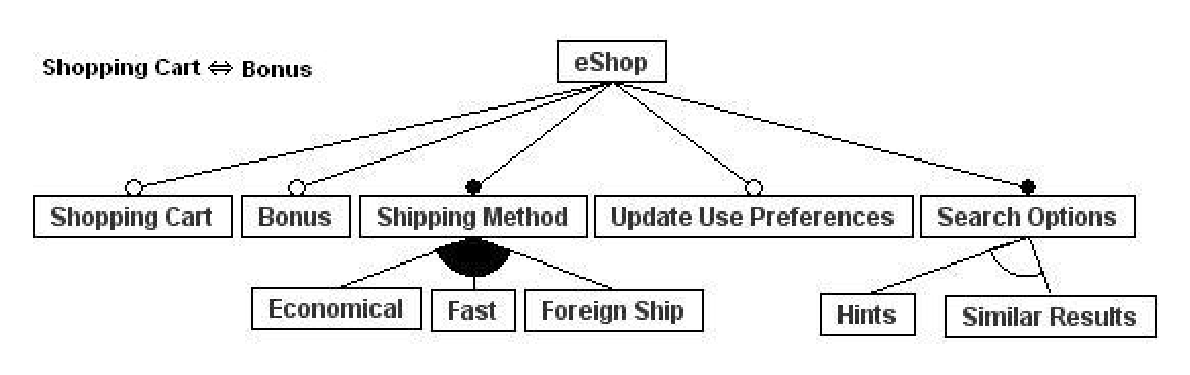
\includegraphics[scale=0.45]{img/eShop-FM.eps}
%   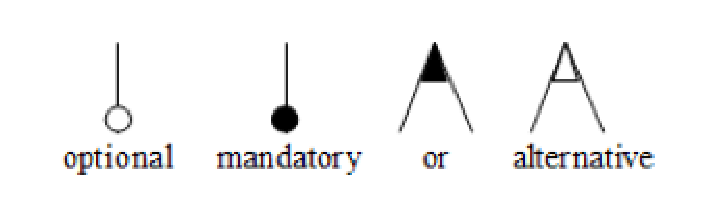
\includegraphics[scale=0.40]{img/fm-notation.eps}
%  \caption{eShop feature model.}
%  \label{fig:eshop-fm}
%  \end{center}
%\end{figure}


%Other approaches are based on use case extensions~\cite{jacobson-reuse-book}, not explored here since they
%require that one use case extension must be defined for each variant. This can result in a huge
%number of use cases that is not suitable for managing activities.


Figure~\ref{fig:pluss-01} depicts the \emph{Buy Product} scenarios written in
the PLUSS notation. Notice that a single artifact is used to represent all valid
configurations related to this scenario, mixing common behavior, variant
behavior, and configuration information (feature selection inside square
brackets). For example, steps 1(a) and 1(b) are never performed together. They
are alternative steps: Step 1(a) will be present only if the \emph{Shopping
Cart} feature is selected, otherwise Step 1(b) will be present. In a similar
way, we have to choose between options (a) and (b) for Step 2 (depending
on whether the \emph{Bonus} feature is selected or not). Finally, Step 6 is
optional and would be present only if the feature \emph{Update User Preference} was selected.

As a consequence, since all possible variants are described in the same
artifact, the behavior of specific products is difficult to understand with the
PLUSS approach. In addition, this tangling between \emph{common} and
\emph{variant} behavior results in maintainability issues: introducing a new product variant
requires changes in several points of existing scenarios. For example, including a
\emph{B2B Integration} feature, which allows the integration between partners in
order to share their warehouses, changes the specification of the \emph{Buy
Product} scenario, enabling the search for product availability in remote
warehouses (a new variant for Step 1) and updating a remote warehouse when the
user confirms the purchase (a new variant for Step 5). Moreover, the inclusion of
this new optional feature also changes the specification of the \emph{Search for
Products} scenario (the search might also be remote). The effort
needed to understand and evolve a product line increases, since the
specification of certain features is scattered through several scenarios,
and each scenario describes several configurations.

% In the PLUSS notation, this kind of relationship between
% features and scenarios is scattered throughout different scenarios.


\begin{figure}[h]
\begin{center}
\begin{scriptsize}
  \texttt{
  \begin{tabular}{|p{0.2in}|p{1.3in}|p{1.3in}|}
   \hline
	Id    & User Action & System Response \\ \hline \hline
       1(a) &Select the checkout option. \mbox{[ShoppingCart]}& Present the
       items in the shopping cart and the amount to be paid. The user can remove
       items from shopping cart. \\  \hline 1(b) & Select the buy product
       option. \mbox{[not ShoppingCart]} & Present the selected product. The
       user can change the quantity of items that he wants to buy. Calculate
       and show the amount to be paid. \\  \hline 2(a) & Select the confirm option. [Bonus]& Request bonus and payment information. \\  \hline 2(b) & Select the confirm option. [not Bonus]& Request payment
       information. \\  \hline 3     & Fill in the requested information and select the proceed option. & Request the shipping method and address.\\  \hline 4     & Select the \$ShippingMethod\$, fill in the destination address and select the proceed option. & Calculate the shipping costs. \\  \hline
       5     & Confirm the purchase. & Execute the order and send a request to the Delivery System in order to dispatch the products. \\  \hline
       (6)     & Select the close session option. \mbox{[Update User
       Preferences]} & Register the user preferences.\\  \hline
  \end{tabular}
  }
\end{scriptsize}
\caption{Buy Products scenarios using PLUSS.}
\label{fig:pluss-01}
\end{center}
\end{figure}



% Section~\ref{sec:evaluation} presents a quantitative study regarded to the PLUSS'
% maintanability issues.

% For example, including a \emph{B2B Integration}
% feature, which allows the integration between partners in order to share their warehouses, might change the specification of the \emph{Buy
% Product} scenario, enabling the search for product availability in remote
% warehouses (a new variant for Step 1) and updating a remote warehouse when the
% user confirms the purchase (a new variant for Step 5). Moreover, the inclusion of
% this new optional feature also changes the specification of the \emph{Search for
% Products} scenario (the search might also be remote). In summary, since the
% behavior of certain features may be spread among several specifications and each
% specification might describe several variants, the effort needed to understand
% and evolve the product line might increase.


Differently, PLUC introduces special tags for representing variation points in
use case scenarios. For example, the VP1 tag in Figure~\ref{fig:pluc-01}, which also
describes the \emph{Buy Products} scenario, denotes a variation point that might
assume the values ``\emph{checkout}'' or ``\emph{buy product}'', depending on
which product is being configured. For each \emph{alternative} or
\emph{optional} step, one tag must be defined. The actual value of each tag is specified in the
\emph{Variation Points} section of a scenario specification.

\begin{figure}[h]
\begin{center}
\begin{scriptsize}
  \texttt{
  \begin{tabular}{{|p{0.05in}p{3in}|}}
  \hline
  & {\bf Buy Products Scenario} \\
  & {\bf Main Flow} \\
  01 & Select [VP1] option \\
  02 & [VP2] \\
  03 & Select the confirm option \\
  04 & [VP3] \\
  05 & Fill in the requested information and select the proceed option \\
  06 & Request the shipping method and address \\
  07 & Select the [VP4] shipping method, fill in the destination address and select the proceed option \\
  08 & Calculate the shipping costs. \\
  09 & Confirm the purchase. \\
  10 & Execute the order and sends a request to the Delivery System in order to dispatch the products \\
  11 & Select the close section option. \\
  12 & \{[VP5] Register the user preferences.\} \\  & \\
  & {\bf Products definition: } \\ & P = (P1, P2) \\ & \\
  & {\bf Variation points: } \\
  &  VP1 =  if (P == P1) then (checkout) \\ & \hspace{0.25in} else (buy product) \\
  & VP2 =  if (P == P1) \\ & \hspace{0.25in}  then (Presents the items in the shopping cart...) \\ & \hspace{0.25in} else (Present the selected product. The user...) \\
  & VP3 =  if (P == P1) \\ & \hspace{0.25in} then ( Requests bonus and payment information.) \\ & \hspace{0.25in} else (Requests payment information.) \\
  & VP4 =  (Economic, Fast) \\
  & VP5 requires (P == P1) \\ \hline
   \end{tabular}
  }
\end{scriptsize}
\caption{Buy Products scenarios using PLUC.}
\label{fig:pluc-01}
\end{center}
\end{figure}

Another kind of tangling occurs in this case. The specifications of common and
variant behavior are separate, but both are tangled with the variation points.
{\color{red}Additionally}, the definition of the SPL members, described using the
same tag notation,  {\color{red} is scattered throughout the \emph{Products
Definition} section of many scenarios (Figure~\ref{fig:pluc-01})}.
{\color{red} Indeed, differently from PLUSS}, there is no explicit
relationship between product configurations and feature models. In the example, two products (P1 and P2) are defined. The first product is configured by an implicit selection of the \emph{Shopping Cart}, \emph{Bonus}, and \emph{Update
User Preferences} features; in contrast to the second product that is not
configured with these features. Since the values of alternative and optional
variation points are computed based on the defined products, instead of specific
features, the inclusion of a new member in the product line might require a deep
review of the scenarios' \emph{Variation Points section}. {\color{red}This problem does not occur in the PLUSS notation}. Moreover, due to the
variation points and the product definitions are spread among several scenario
specifications, it is hard and time consuming to keep consistent the
relationships between them. Finally, the same definitions (product configuration
and variation points) are often useful to manage variabilities in other
artifacts, such as design and source code, implying that PLUC
requires the replication of such definitions in different SPL views.

In conclusion, both PLUSS and PLUC do not present a clear separation between
variability assets and scenario specifications, which compromises the
evolution of a SPL. Besides that, both approaches rely on simple
variability techniques: filtering optional steps in scenarios, or syntactic
changes of tag values based on product definition. In this sense, according to the terminology
presented in~\cite{Kastner:2008aa}, they can be classified as \emph{annotated
techniques}, which are not suitable for modularizing the crosscutting nature of certain
features, have poor legibility, and lead to lower
maintainability~\cite{Alves:2006aa,Kastner:2008aa}.

% For this reason, Pohl et al. argued that the
% variability management concern should be separated from the other SPL
% assets~\cite{Pohl:2005aa}. However, besides the use of independent models for
% representing the variability concern, it is also necessary concrete descriptions
% of the composition processes used to generate specific products.


% this case, in order to support the automatic derivation of product specific
% artifacts, it is necessary not only to have a more precise definition of each
% language used to describe product line artifacts and the variability management
% concern, but also to formalize the weaving processes used to combine them.
%
% The
% PLUSS and PLUC approaches fail in this direction, since Eriksson et al. defines
% the metamodel of PLUSS notation~\cite{eriksson-splc-2005}, but do not describe
% which languages and processes are used for relating use case scenarios to feature
% models. Likewise, although Fantechi et al. describe the formal semantics of
% PLUC~\cite{fantechi-splc-2004}, this approach does not separate variability
% management from use case scenarios.

% Next section describes our approach, named as Scenario Variability as
% Crosscutting Mechanisms (SVCM), which deals with scenario variability
% management by means of the composition of different artifacts. A key
% characteristic found in SVCM is that each involved artifact has a clear and
% specific contribution to the SPL engineering.

% Although in this paper we are focus on use
% case scenarios, the idea of separating product line artifacts from variability
% management (using feature models, product configurations, and configuration
% knowledge) is also applied to other SPL views. 
% -------------------------------------------------------------------------
% Section: Modeling the Variability Mechanisms
% ------------------------------------------------------------------------
\section{SVCM Approach}
\label{sec:svmc}

To solve the problems mentioned in the previous section, we introduce now our
approach for modeling variabilities in use case scenarios, which was named
\emph{Modeling Scenario Variability as Crosscutting Mechanisms} (MSVCM). It
improves the separation of concerns between variability management and scenario
specifications, dealing with scenario variability as a composition of different
artifacts: SPL use case model, feature model, product configuration,
and configuration knowledge.

Motivated by the Masuhara and Kiczales (MK) work~\cite{Masuhara:2003aa}, our
approach for \textbf{scenario variability management} is based on a weaving
process that takes as input the aforementioned artifacts, which crosscut
each other with respect to the resulting product specific use case model
(Figure~\ref{fig:weave-process}). Combining these input artifacts, it is possible
to represent the sources of variability that we are interested in:
\emph{variability in function}, \emph{variability in data}, and \emph{variability in
control flow}~\cite{Bachmann:2001aa}.

\begin{figure}[htb]
 \begin{center}
  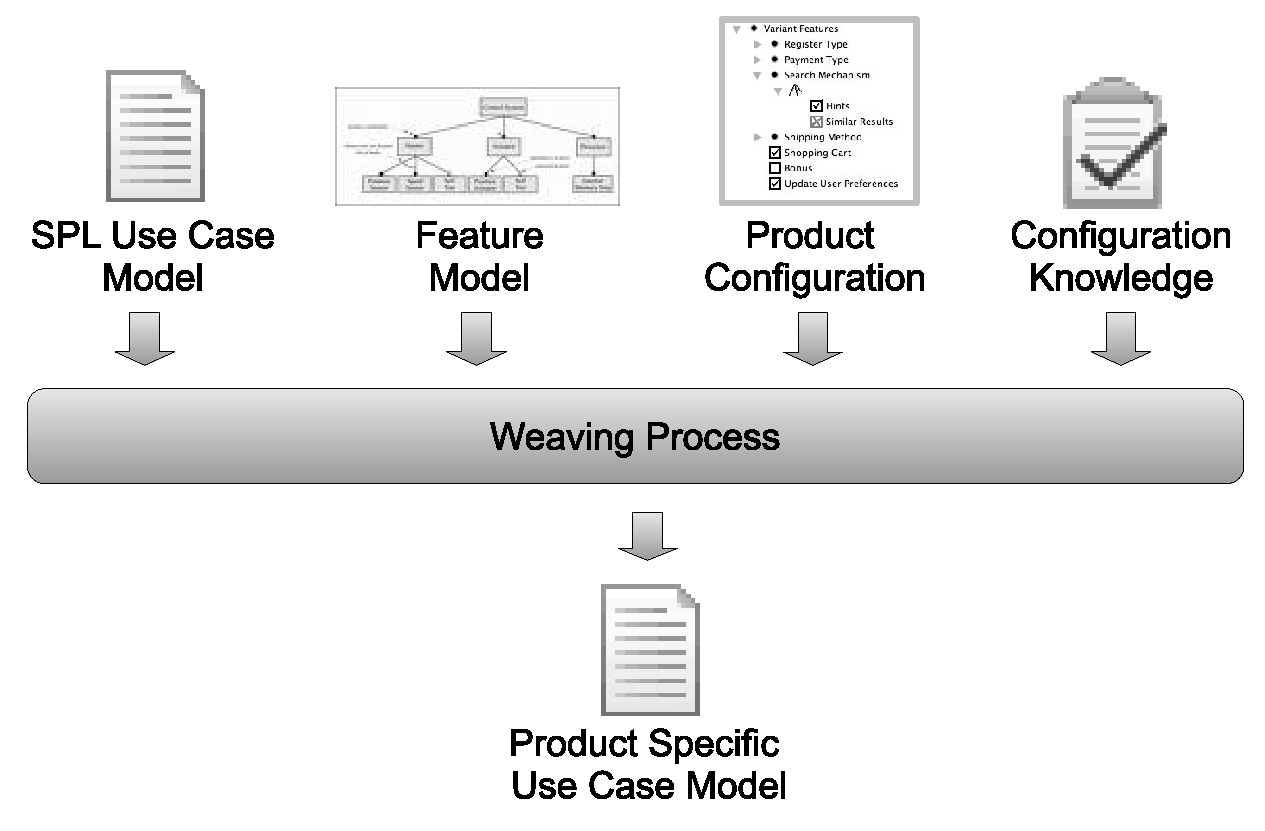
\includegraphics[scale=0.30]{img/weave-process2.eps}
  \caption{Overview of our weaving process.}
  \label{fig:weave-process}
  \end{center}
\end{figure}

\newpage

{\color{blue}The semantics of the weaving process (and the
meta-model of the input and output languages) are described using the Haskell
programming language. This led to concise descriptions and kept our model close
to the MK work, where their weaving processes are specified using Scheme---
another functional programming language. The choice for Haskell was motivated by
several factors, such as improved readability and our background in the language.
The resulting source code is available at a web site~\cite{SPG:site}.} In what follows, we detail our approach showing
how it can be used to specify the motivating example. Several artifacts of each
input model are shown; mentioning the contribution of these models to the whole
weaving process.

% {\color{red} With
% respect to the supporting tools, instances of the input models are specified
% using \emph{widespread} tools, and then imported to our variability
% management environment. In this section, we also explain which are these tools and present
% the layered architecture of the Haskell libraries used in our environment.} After
% that, in Section~\ref{sec:modeling-framework} we describe the semantics of our
% approach using a slight customization of the MK framework.



\subsection{Feature model}

Feature models have an important contribution to our weaving process, since they
are used for checking if a product configuration is a valid member of the product
line. We have implemented specific functions in Haskell to deal with
this kind of validation. Basically, these functions verify if all constraints defined in
a feature model are satisfied by a product configuration. 

The code fragment below presents the signature of the \emph{topmost} function
for checking instances of a feature model. It states that
\texttt{checkConfiguration} takes as input a feature model (\emph{FM}) and a
product configuration (\emph{PC}), returning all constraints that a
\emph{PC} does not satisfy. If a \emph{PC} complies with the \emph{constraints}, the
function returns an empty list.

\begin{hscode}\SaveRestoreHook
\column{B}{@{}>{\hspre}l<{\hspost}@{}}%
\column{E}{@{}>{\hspre}l<{\hspost}@{}}%
\>[B]{}\Varid{checkConfiguration}\mathbin{::}\Conid{FM}\to \Conid{PC}\to \Conid{ErrorList}{}\<[E]%
\ColumnHook
\end{hscode}\resethooks

Going into details, the \texttt{checkConfiguration} function traverses two
\emph{rose trees}~\cite{Hinze:2007aa}, representing both feature model and
product configuration, at the same time that it calls specific functions for
checking the rules applied for each type of feature relationship
(mandatory, exclusive or, inclusive or) and constraints. 

{\color{blue}
Although we are not proposing a new notation for feature modeling, we
had to create specific data types for feature models in Haskell.  The same was
true for the other input models of our weaving process. For instance, the code
bellow shows the feature model data type. It basically consists of a root feature
and a list of global constraints. Due to lack of space, in this paper we do not
present all input model data types.

\begin{hscode}\SaveRestoreHook
\column{B}{@{}>{\hspre}l<{\hspost}@{}}%
\column{3}{@{}>{\hspre}l<{\hspost}@{}}%
\column{9}{@{}>{\hspre}l<{\hspost}@{}}%
\column{25}{@{}>{\hspre}c<{\hspost}@{}}%
\column{25E}{@{}l@{}}%
\column{E}{@{}>{\hspre}l<{\hspost}@{}}%
\>[B]{}\mathbf{data}\;\Conid{FeatureModel}\mathrel{=}\Conid{FeatureModel}\;\{\mskip1.5mu {}\<[E]%
\\
\>[B]{}\hsindent{9}{}\<[9]%
\>[9]{}\Varid{root}\mathbin{::}\Conid{Feature},{}\<[E]%
\\
\>[B]{}\hsindent{9}{}\<[9]%
\>[9]{}\Varid{constraints}\mathbin{::}[\mskip1.5mu \Conid{Constraint}\mskip1.5mu]{}\<[E]%
\\
\>[B]{}\mskip1.5mu\}{}\<[E]%
\\
\>[B]{}\mathbf{data}\;\Conid{Feature}\mathrel{=}\Conid{Feature}\;{}\<[25]%
\>[25]{}\{\mskip1.5mu {}\<[25E]%
\\
\>[B]{}\hsindent{3}{}\<[3]%
\>[3]{}id\mathbin{::}{}\<[9]%
\>[9]{}\Conid{Id},{}\<[E]%
\\
\>[B]{}\hsindent{3}{}\<[3]%
\>[3]{}\Varid{name}\mathbin{::}\Conid{Name},{}\<[E]%
\\
\>[B]{}\hsindent{3}{}\<[3]%
\>[3]{}\Varid{featureType}\mathbin{::}\Conid{FeatureType},\mbox{\onelinecomment  (optional, mandatory)}{}\<[E]%
\\
\>[B]{}\hsindent{3}{}\<[3]%
\>[3]{}\Varid{featureGroup}\mathbin{::}\Conid{Group},\mbox{\onelinecomment  (none, ior, xor)}{}\<[E]%
\\
\>[B]{}\hsindent{3}{}\<[3]%
\>[3]{}\Varid{children}\mathbin{::}[\mskip1.5mu \Conid{Feature}\mskip1.5mu]{}\<[E]%
\\
\>[B]{}\mskip1.5mu\}{}\<[E]%
\ColumnHook
\end{hscode}\resethooks
}
 
Additional functions were defined for importing feature models, generated by the
\emph{Feature Modeling Plugin} (FMP)~\cite{Czarnecki:2004aa}, to our
environment. In the remainder of this section, we consider the \emph{eShop}
feature model introduced in the motivating example (Figure~\ref{fig:eshop-fm}). 

%For
%instance, {\color{blue}Based on the feature model of Figure~\ref{fig:eshop-fm},
%the \emph{Shopping Cart}, \emph{Bonus} and \emph{Update User Preferences}
%features are optional; on the other hand, the \emph{Shipping Method} feature is
%mandatory and all products have to be configured with at least one of its child.
%Additionally, the restriction $Shopping\ Cart\ \Leftrightarrow\ Bonus$ states
%that all products configured with the shopping cart feature must also be
%configured with the bonus feature. More details about feature modeling can be
%found elsewhere~\cite{Gheyi:2006aa,Czarnecki:2000aa}.}

\subsection{SPL use case model}\label{sub:spl-uc}

This artifact defines scenarios that describe the expected behavior of the SPL's
members. Scenarios might be optional, have parameters, and change (advice) the
behavior of other scenarios. A use case model is composed by \emph{use cases} and
\emph{aspectual use cases}. A use case has a name, a description and a list of
scenarios, which are composed by a sequence of steps (pairs of \emph{User action x
System response}). An aspectual use case has a name and a list of advices, which
can be used to extend the behavior of existing scenarios.

Differently from PLUSS, which directly relates alternative and
optional steps to features, in our approach \emph{feature} and \emph{use case
models} are syntactically independent from each other. There is no direct
association joining these models and all relationships between them are kept by
the configuration knowledge (Section~\ref{sub:configuration-knowledge}).
 Actually, the weaving process, whose semantics are presented in
 Section~\ref{sec:modeling-framework}, is responsible for binding the variation
 points defined in the SPL use case model. In order to do that, other assets
 (such as product configurations and configuration knowledge) have to be
 consider.

{\color{blue} Regarding tool support, instances of the use case model can
be written in any text editor that is able to export documents using a specific
XML format\footnote{Templates are available for Microsoft Word.}. Additional functions were
developed for parsing these documents to the abstract data type of our use case
model.}

In this running example, we consider the following scenarios and advices:

{\bf Proceed to Purchase:} this mandatory scenario
(Figure~\ref{fig:proceed-to-checkout}) specifies the common behavior that is
required for confirming a purchase. Instances of the product line must be
configured with this scenario. 
Notice that a parameter (\emph{SM}) is referenced in Step P2. 
This parameter allows the reuse of the \emph{Proceed to
Purchase} scenario for different configurations of the \emph{Shipping Method} feature. {\color{red} Parameters 
are also supported in PLUSS and PLUC. However, in these approaches parameters are directly related to features or members of the product line.}

The annotation \mbox{\texttt{[CustomerPreferences]}} (Step P3) is
another variation point of \emph{Proceed to Purchase} scenario. This annotation, also assigned to the Step S3 of \emph{Search for Products} (Figure~\ref{fig:search-products-flow}), reveals points in the specification that are related to the customer preferences. Since pointcuts can make references to annotations, the advice \emph{Register User Preferences} (Figure~\ref{fig:register-preferences-flow}) extends the behavior of \emph{Proceed to Purchase} after Step P3. Note that our annotations just reveal variation points, which means that annotated steps are \emph{obliviousness} about which features extend the corresponding behavior. 


\begin{figure}[h]
\begin{scriptsize}
  \texttt{
   \begin{tabular}{l}
   	 {\bf Id: SC01} 	\\
     {\bf Description:} Proceed to purchase\\
   \end{tabular}
  \begin{center}
  \begin{tabular}{|p{0.1in}|p{1.4in}|p{1.4in}|}
   \hline
       Id & User Action  & System Response \\ \hline \hline
       P1 & Fill in the requested information and select the proceed option.  & Request the shipping method and address.\\  \hline
       P2 & Select one of the available shipping methods (\mbox{<SM>}),
       fill in the destination address and proceed. & Calculate the shipping costs. \\  \hline P3 & Confirm the purchase. & Execute the order and send a request to the Delivery System to dispatch the products.
       \mbox{[CustomerPreferences]} \\  \hline
  \end{tabular}
  \end{center}
  }
\end{scriptsize}
\caption{Proceed to purchase scenario.}
\label{fig:proceed-to-checkout}
\end{figure}

{\bf Buy Product:} this advice (Figure~\ref{fig:buy-product-scenario}) enables a
customer to buy specific goods from an on-line shopping store. It is only
available in the product line members that are {\bf not} configured with the
\emph{Shopping Cart} and \emph{Bonus} features. The effect of this advice is to
introduce an optional behavior {\bf before} the join points identified in its
\emph{pointcut} clause. In this case, the Step P1 defined in the \emph{Proceed to
Purchase} scenario. {\color{red} Therefore, the \emph{pointcut} clause can refer either to step ids or
step annotations (as explained before). However, we encourage the definition of
pointcuts based on annotations, since they mitigate the problem
of fragile pointcuts. This problem occurs because changes in the order of
steps might break pointcuts.}
 
\begin{figure}[h]
\begin{scriptsize}
  \texttt{
   \begin{tabular}{l}
   	 {\bf Id: ADV01} 	\\
     {\bf Description:} Buy a specific product\\
     {\bf Before:}  P1
   \end{tabular}
  \begin{center}
  \begin{tabular}{|p{0.1in}|p{1.4in}|p{1.4in}|}
   \hline
       Id & User Action  & System Response \\ \hline \hline
       B1 & Select the buy product option.  & Present the selected product. The user can change the quantity of items he wants to buy. Calculate and show the amount to be paid. \\  \hline
       B2 & Select the confirm option. &  Request payment information. \\  \hline
    \end{tabular}
  \end{center}
  }
\end{scriptsize}
\caption{Buy product advice.}
\label{fig:buy-product-scenario}
\end{figure}

{\bf Buy Products with Shopping Cart and Bonus:} this advice
(Figure~\ref{fig:buy-product-changing-flow}) allows purchasing products
that have been previously added to a shopping cart. It extends the
behavior of the \emph{Proceed to Purchase} scenario by introducing the specific
behavior required by the \emph{Shopping Cart} and
\emph{Bonus} features. So, this advice is required by products that
are configured with both \emph{Shopping Cart} and \emph{Bonus} features.

\begin{figure}[h]
\begin{scriptsize}
  \texttt{
   \begin{tabular}{l}
   	 {\bf Id: ADV02} 	\\
     {\bf Description:} Buy products using a shopping-cart\\
     {\bf Before:} P1
   \end{tabular}
  \begin{center}
   \begin{tabular}{|p{0.1in}|p{1.4in}|p{1.4in}|}
   \hline
       Id & User Action & System Response \\ \hline \hline
       C1 & Select the checkout option.  & Present the items in the shopping cart and the amount to be paid. The user can remove items from the shopping cart. \\  \hline
       C2 & Select the confirm option. & Request bonus and payment information. \\  \hline
  \end{tabular}
  \end{center}
  }
\end{scriptsize}
\caption{Buy products with shopping cart advice.}
\label{fig:buy-product-changing-flow}
\end{figure}

{\bf Search for Products:} this mandatory scenario
(Figure~\ref{fig:search-products-flow}) allows a customer to search for products.
In order to save space, we only present Step S3, which performs a search based on
the input criteria. {\color{red}Note that, similarly to the Step P3 shown in
Figure~\ref{fig:proceed-to-checkout}, this step is also assigned to the
\mbox{\texttt{ [CustomerPreferences]}} annotation. Therefore, any advice that
points to this annotation extends, at least, the behavior of \emph{Proceed to Purchase} and
\emph{Search for Product} scenarios.}

\begin{figure}[ht]
\begin{scriptsize}
  \texttt{
   \begin{tabular}{l}
   	 {\bf Id: SC02} 						\\
     {\bf Description:} Search for products. \\
   \end{tabular}
  \begin{center}
   \begin{tabular}{|p{0.1in}|p{1.4in}|p{1.4in}|}
   \hline
       Id & User Action &  System Response \\ \hline \hline
       \ldots & \ldots  & \ldots \\  \hline
       S3 & Inform the search criteria. &  Retrieve the products that satisfy the search criteria. Show a list with the resulting products. [CustomerPreferences] \\  \hline
  \end{tabular}
  \end{center}
  }
\end{scriptsize}
\caption{Search for products scenario.}
\label{fig:search-products-flow}
\end{figure}



{\bf Register User Preferences:} this advice
(Figure~\ref{fig:register-preferences-flow}) updates the user preferences based
on the user's history of searches and purchases. Its behavior can be started {\bf
after} any step assigned to the \texttt{[CustomerPreferences]} (see the
\emph{pointcut} clause) annotation and is available in products that are
configured with the \emph{Update User Preferences} feature.

\begin{figure}[h]
\begin{scriptsize}
  \texttt{
   \begin{tabular}{l}
   	 {\bf Id: ADV03} 	\\
     {\bf Description:} Register user preferences.\\
     {\bf After}: [CustomerPreferences] \\
   \end{tabular}
  \begin{center}
   \begin{tabular}{|p{0.1in}|p{1.4in}|p{1.4in}|}
   \hline
       Id & User Action &  System Response \\ \hline \hline
       R1 & - &  Update the preferences based on the search results or purchased items. \\  \hline
  \end{tabular}
  \end{center}
  }
\end{scriptsize}
\caption{Register user preferences.}
\label{fig:register-preferences-flow}
\end{figure}

{\color{red} At this point we are able to present some remarks related to our use
case model. As discussed in Section~\ref{sec:problem}, PLUSS and PLUC represent
all valid configurations of a scenario in a single artifact. Differently, using
our approach, we could separate the common behavior required to confirm a
purchase (the base scenario \emph{Proceed to Purchase}) from its variants,
specified in the \emph{Buy Product} and \emph{Buy Product with Shopping Cart}
advices. {\color{blue}This allows our specifications to evolve according to the
\emph{Open-Closed} principle~\cite{Meyer:2000aa}; which means that, in our
approach, introducing new product variants require more extensions than changes
to the base scenarios.} 

Moreover, in this section we have described several
scenarios as being optional or mandatory, being important to emphasize
that, in our approach, this kind of information is not specified in the use case
model. Actually, it is necessary to consider the relationships between features
and scenarios, represented in the configuration knowledge, in order to be aware
of which scenarios are present in a specific product configuration. Finally,
since different advices can make references to a same joinpoint,  interferences
between advices may occur. Nevertheless, the weaving process evaluates each advice in
a sequence defined by the configuration knowledge. For this reason, interferences
between advices are deterministic and do not require specific constructs in the
use case model to deal with them.}

\subsection{Configuration knowledge}\label{sub:configuration-knowledge}

{\color{red} This artifact corresponds to a list of configuration items, which
relates feature expressions to tasks (or transformations) used for automatically generating a
SPL member. Consequently, the configuration knowledge guides the weaving
process}. For this running example, the configuration knowledge shown in
Table~\ref{tab:eshop-ck} enforces that

\begin{itemize}
\item Both \emph{Proceed to Purchase} (SC01) and \emph{Search for Products}
(SC02) scenarios are mandatory, since their selection is related to the
(mandatory) root feature of the \emph{eShop} product line;

\item The \emph{Buy Product} advice (ADV01) is used in the composition of
products that do not have been configured with both \emph{Shopping Cart} and \emph{Bonus}
features--- if both features were selected for a product, it would be configured
with the \emph{Buy Product with Cart} advice (ADV02). Remember that there is a
mutual dependency between \emph{Shopping Cart} and \emph{Bonus} features. As a
consequence, no product can be configured with just one of them;

\item The \emph{Register User Preferences} advice (ADV03) is not used in a
product composition unless the \emph{Update User Preferences} feature has been
selected; and

\item References to the ``SM'' parameter are bound to the
selected alternatives of the \emph{Shipping Method} feature.

\end{itemize}

\begin{table}[htb]
\begin{small}
\begin{tabular}{|lp{1.4in}|}
\hline
Feature Expression  						& Tasks					 \\ \hline \hline

\multirow{2}{*}{eShop}						& select scenario {\bf SC01} \\
											& select scenario {\bf SC02} \\	 \hline
{\bf not} (Shopping Cart {\bf and} Bonus) 	& evaluate advice {\bf ADV01} \\ \hline 
(Shopping Cart {\bf and} Bonus) 		& evaluate advice {\bf ADV02} 	\\   \hline
Update User Preferences 				& evaluate advice {\bf ADV03} \\     \hline 
\multirow{2}{*}{Shipping Method}		& bind {\bf SM} to {\bf Shipping} \\  
										& {\bf Method}\\ \hline
								
\end{tabular}
\end{small}
\caption{Example of configuration knowledge}
\label{tab:eshop-ck}
\end{table}

{\color{red}Three different tasks are shown
in Table~\ref{tab:eshop-ck}: \emph{select scenario}, \emph{evaluate advice}, and
\emph{bind parameter}. According to Bachmann et
al.~\cite{Bachmann:2001aa}, the first type of task deals with the source of
variability named as \emph{variation in function}, being responsible for
selecting scenarios; the second one deals with \emph{variation in control flow},
being responsible for composing advices at specific joinpoints; and the last one
deals with \emph{variation in data}, being responsible for binding parameters to
features.} 

{\color{red} The semantics of these tasks are described as crosscutting mechanisms
in Section~\ref{sec:modeling-framework}. Besides that, the configuration knowledge data type is shown bellow. As explained before, it is a list of configuration items, which relate feature expressions to
\emph{tasks}. Actually, the type \texttt{Task} is a synonymous for the
family of functions that receive a \emph{SPL use case model} ($SPL$) and a \emph{product
specific use case model} ($SPLMember$) as parameters; and then returns a
refinement of the product specific model.}
 
 % \begin{small}
 \begin{hscode}\SaveRestoreHook
\column{B}{@{}>{\hspre}l<{\hspost}@{}}%
\column{3}{@{}>{\hspre}l<{\hspost}@{}}%
\column{E}{@{}>{\hspre}l<{\hspost}@{}}%
\>[B]{}\mathbf{type}\;\Conid{ConfigurationKnowledge}\mathrel{=}[\mskip1.5mu \Conid{Configuration}\mskip1.5mu]{}\<[E]%
\\[\blanklineskip]%
\>[B]{}\mathbf{data}\;\Conid{Configuration}\mathrel{=}\Conid{Configuration}\;\{\mskip1.5mu {}\<[E]%
\\
\>[B]{}\hsindent{3}{}\<[3]%
\>[3]{}\Varid{exp}\mathbin{::}\Conid{FeatureExpression},{}\<[E]%
\\
\>[B]{}\hsindent{3}{}\<[3]%
\>[3]{}\Varid{tasks}\mathbin{::}[\mskip1.5mu \Conid{Task}\mskip1.5mu]{}\<[E]%
\\
\>[B]{}\mskip1.5mu\}{}\<[E]%
\\[\blanklineskip]%
\>[B]{}\mathbf{type}\;\Conid{Task}\mathrel{=}(\Conid{SPL}\to \Conid{SPLMember})\to \Conid{SPLMember}{}\<[E]%
\ColumnHook
\end{hscode}\resethooks

{\color{red}Note that feature expressions have to be written in propositional
logic, because it is necessary to express, for example, that the \emph{Buy Products} advice will be evaluated iff the feature expression {\bf ``not ShoppingCart and Bonus''} is true for a specific product configuration.

Indeed, the \emph{weavingProcess} function, whose source code is presented bellow, behaves like a generator that applies 
the appropriate list of tasks ($ts$) for a given product configuration. This means 
that, first of all, it is necessary to verify  ($eval\ pc\ (exp\ c)$) which expressions ($exp\ c$) 
are valid for a specific product configuration ($pc$). After that, the
$stepRefinement$ function composes the sequence of tasks that must be applied. 

\begin{hscode}\SaveRestoreHook
\column{B}{@{}>{\hspre}l<{\hspost}@{}}%
\column{4}{@{}>{\hspre}l<{\hspost}@{}}%
\column{5}{@{}>{\hspre}l<{\hspost}@{}}%
\column{E}{@{}>{\hspre}l<{\hspost}@{}}%
\>[B]{}\Varid{weavingProcess}\;\Varid{spl}\;\Varid{fm}\;\Varid{pc}\;\Varid{ck}\mathrel{=}{}\<[E]%
\\
\>[B]{}\hsindent{4}{}\<[4]%
\>[4]{}\Varid{stepRefinement}\;[\mskip1.5mu (\Varid{t}\;\Varid{spl})\mid \Varid{t}\leftarrow \Varid{ts}\mskip1.5mu]\;\Varid{empty}{}\<[E]%
\\
\>[B]{}\hsindent{4}{}\<[4]%
\>[4]{}\mathbf{where}{}\<[E]%
\\
\>[4]{}\hsindent{1}{}\<[5]%
\>[5]{}\Varid{ts}\mathrel{=}\Varid{concat}\;[\mskip1.5mu \Varid{tasks}\;\Varid{c}\mid \Varid{c}\leftarrow \Varid{ck},\Varid{eval}\;\Varid{pc}\;(\Varid{exp}\;\Varid{c})\mskip1.5mu]{}\<[E]%
\\
\>[4]{}\hsindent{1}{}\<[5]%
\>[5]{}\Varid{empty}\mathrel{=}(\Varid{emptyInstance}\;\Varid{spl}\;\Varid{pc}){}\<[E]%
\\
\>[4]{}\hsindent{1}{}\<[5]%
\>[5]{}\Varid{stepRefinement}\;\Varid{l}\;\Varid{m}\mathrel{=}\mathbin{...}{}\<[E]%
\ColumnHook
\end{hscode}\resethooks
 
As a consequence, supposing the list of tasks
 
$ts=[select(SC01),evaluate(ADV01),evaluate(ADV02)]$,
 
the semantics of this hypothetical product would be given by: $p\ =\  f\ (spl,\ g\ (spl,\ h))$, where:
\begin{eqnarray*}
h  & = & (select\ SC01)\ spl\ emptyInstance \\
g  & = & (evaluate\ ADV01) \\
f   & = & (evaluate\ ADV02) \\
\end{eqnarray*}

{\color{red}The previous input models are specified during the domain
engineering phase of SPL development~\cite{Clements:2001aa,Pohl:2005aa}. The next
one, on the other hand, is supposed to be designed whenever a specific product
has to be generated. }

\subsection{Product configuration}\label{subsub:pc}

This artifact identifies a specific SPL member, which is characterized by a
configuration of features. One important property is that each product
configuration must comply to a feature model (the selected features must obey
the feature model relationships and constraints).

{\color{red}In our environment, we also use the FMP
tool~\cite{Czarnecki:2004aa} for configuring individual products. Then,
we parse such configurations to our
environment, instantiating the abstract representations of the product
configuration input model. Actually, the abstract representation of a product
configuration is basically a tree representing the selected features. For the
\emph{eShop} example, two possible configurations are presented in
Figure~\ref{fig:product-config-01-02}.}

 \begin{figure}[h]
 \begin{center}
  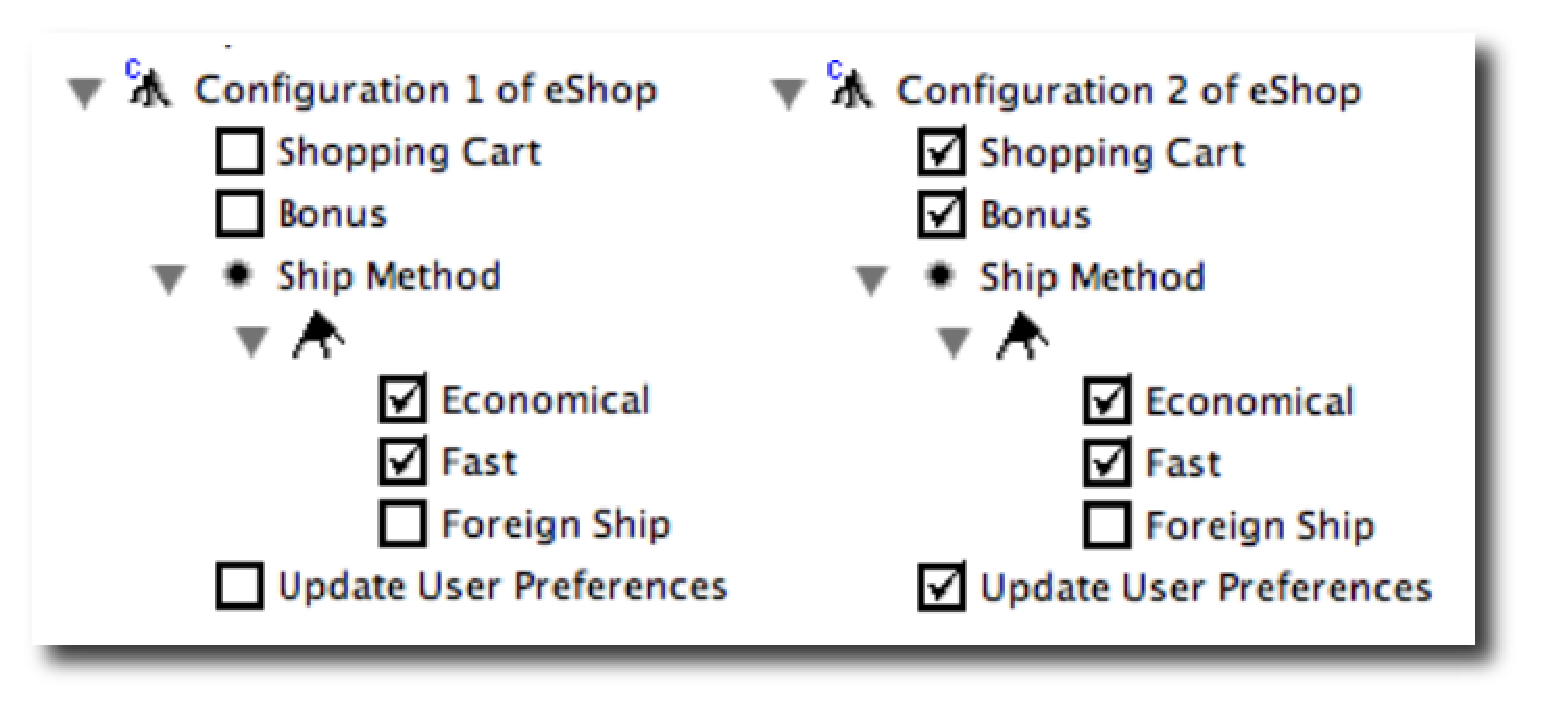
\includegraphics[scale=0.33]{img/pc-04.eps}
   \caption{Examples of product configurations.}
  \label{fig:product-config-01-02}
  \end{center}
\end{figure}

The first configuration (on the left side of the
Figure~\ref{fig:product-config-01-02}) defines a product that does not have support for
\emph{Shopping Cart}, \emph{Bonus} and \emph{Update User Preferences}.
Additionally, it supports only the economical and fast shipping methods. The
second configuration is more complete, being configured with the features
\emph{Shopping Cart}, \emph{Bonus}, and \emph{Update User Preferences}.

{\color{red} As explained in the previous section, the features selected to a specific product
(represented as a product configuration) identify which \emph{tasks} (or
transformations) must be performed in order to generate the corresponding SPL
member. 
Figure~\ref{fig:resulting-scenarios} depicts the resulting scenarios after evaluating the configuration knowledge of
Table~\ref{tab:eshop-ck} and considering the second configuration of
Figure~\ref{fig:product-config-01-02}. According to what was explained in the
previous section, such a configuration requires: 

\begin{enumerate} 
 \item The selection of \emph{Proceed to Purchase} and \emph{Search for Product} scenarios. This selection is directly responsible 
for the resulting scenarios shown in Figure~\ref{fig:resulting-scenarios}. 
  
 \item The evaluation of \emph{Buy Products with Cart} advice. The result of this evaluation is the introduction of the 
first two steps in the resulting specification of the \emph{Proceed to Purchase} scenario. 
 
 \item The evaluation of \emph{Register User Preferences} advice. The result of this evaluation is the introduction of the last steps 
{\color{blue}on} both \emph{Search for Products} and \emph{Proceed to
Purchase} scenarios.

 \item The binding of the \emph{SM} parameter to the selected options of the \emph{Shipping Method} feature. This binding is responsible for 
 setting the options \emph{Economical} and \emph{Fast} in the fourth step of the
 resulting \emph{Proceed to Purchase} scenario.

\end{enumerate}
}
 
\begin{figure}[h]
\begin{scriptsize}
   \texttt{
     \begin{tabular}{l}
   	 {\bf Scenario:} Search for products.\\
      \end{tabular}
   \begin{center}
     \begin{tabular}{|p{0.1in}|p{1.45in}|p{1.4in}|} \hline
      id & User Action  & System Response \\ \hline \hline
       \ldots & \ldots  & \ldots \\  \hline
        3 & Inform the search criteria. &  Retrieve the products that satisfy the search criteria. Show a list with the resulting products. \\   \hline
        4 & - &  Update the preferences based on the search results or purchased items \\\hline 
     \end{tabular}
   \end{center}
   \begin{tabular}{l}
   	 \\
	 {\bf Scenario:} Proceed to purchase.\\
      \end{tabular}
   \begin{center}
     \begin{tabular}{|p{0.1in}|p{1.40in}|p{1.40in}|} \hline
       id & User Action  & System Response \\ \hline \hline
       1 & Select the checkout option.  & Present the items in the shopping
       cart and the amount to be paid. The user can remove items from the
       shopping cart. \\ \hline
       2 & Select the confirm option. & Request bonus and payment information. \\ \hline
       3 & Fill in the requested information and
       select the proceed option.  & Request the shipping method and address.\\ \hline
       4 & Select one of the available shipping methods {\bf (Economical, Fast)}, fill
       in the destination address and proceed. & Calculate the shipping
       costs.\\ \hline
       5 & Confirm the purchase. & Execute the order and send a
       request to the Delivery System to dispatch the products. \\ \hline
 	6 & - &  Update the preferences based on the search results or purchased
 	   items. \\ \hline
    \end{tabular}
   \end{center}
   }
\end{scriptsize}
\caption{Resulting scenarios of the example}
\label{fig:resulting-scenarios}
\end{figure}	

The next section details the semantics of our
weaving process, modeling each source of scenario variability as a crosscutting 
mechanism.

%=====================================================
% TOOL Support
%=====================================================

% \subsection{Tool support}
% 
% {\color{red}As explained before, we are using external tools for specifying 
% features models, use case models, and product configurations. Therefore, only 
% the configuration knowledge is written using the tool support
% {\color{blue}developed for testing the ideas presented in this paper.} 
% 
% Besides allowing the users to specify configuration models, the tool 
% parses the input models from XML documents and starts the weaving process.
% Figure~\ref{fig:graphical-environment} shows the graphical environment that
% integrates these functionalities.
% 
% \begin{figure}[h]
%  \begin{center}
%   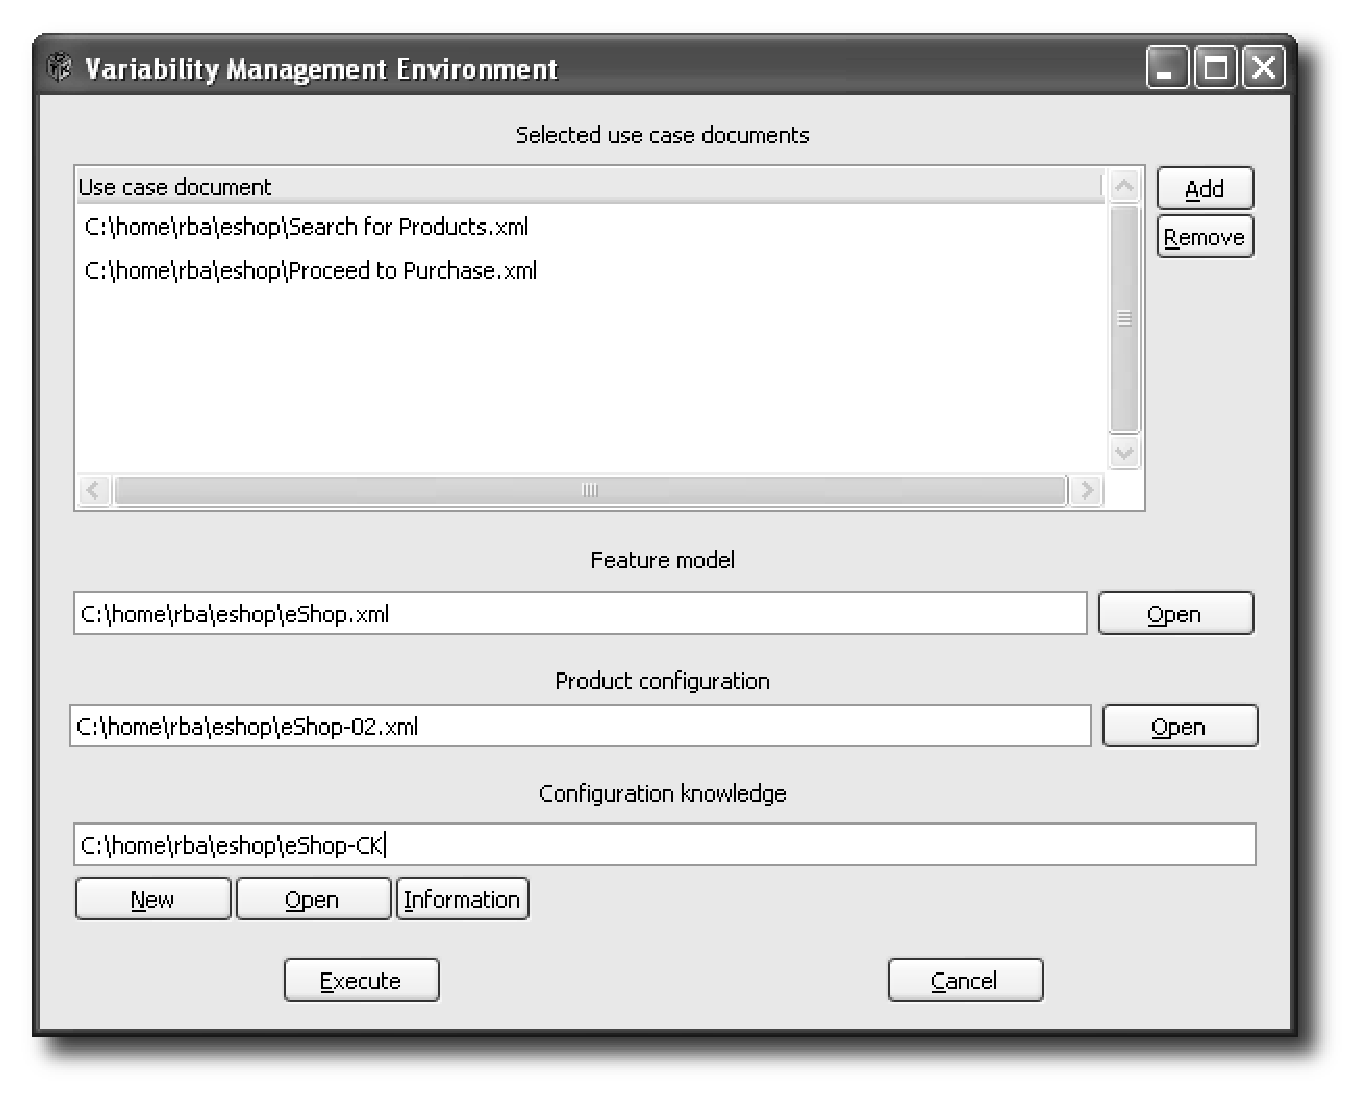
\includegraphics[scale=0.40]{img/msvcmTool.eps}
%    \caption{Weaving process' graphical environment.}
%   \label{fig:graphical-environment}
%   \end{center}
% \end{figure}
% 
% Similar to the weaving process, detailed in the next section, the tool support
% was also developed in Haskell, reusing common libraries for parsing XML documents
% (HXT) and graphical user interface (gtk2hasell). One overview of the major
% libraries and tools is shown in Figure~\ref{fig:haskell-libraries}.}
% 
% \begin{figure}[h]
%  \begin{center}
%   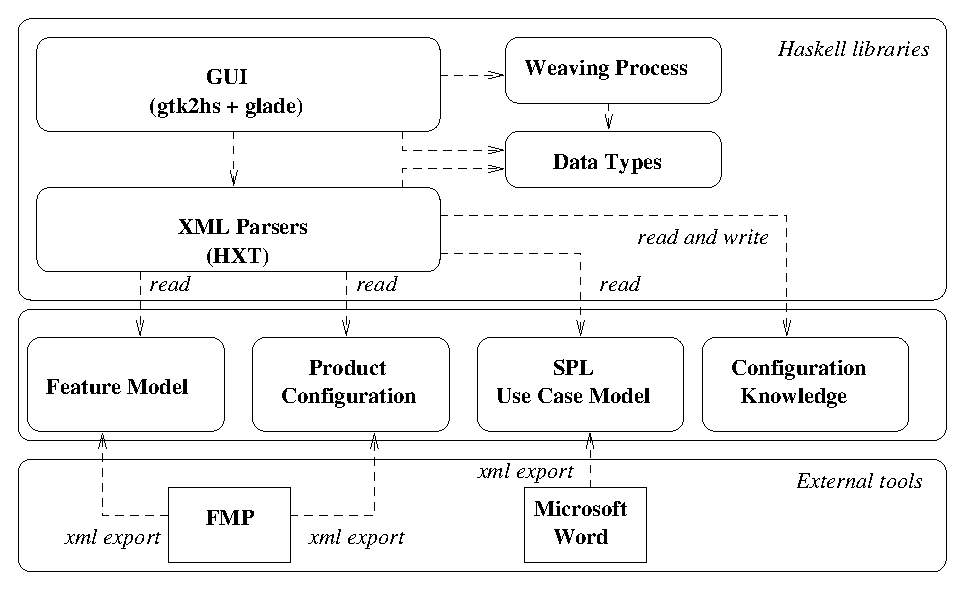
\includegraphics[scale=0.55]{img/architecture.eps}
%    \caption{Haskell libraries and external tools.}
%   \label{fig:haskell-libraries}
%   \end{center}
% \end{figure}


%There is no artifact similar to our configuration knowledge in
%PLUSS and PLUC approaches. As a consequence, introducing new variants of existing
%features in these techniques usually propagates changes throughout many
%scenarios.


%=================================================================
% Semantica do configuration knowledge
%=================================================================
% \begin{figure*}[hbt]
%  \begin{code}
%   (|->) :: a -> b -> (a,b) -- just a 'syntactic sugar' to build pairs
%   l |-> r = (l,r)
%
%   conf1 = Configuration (``eShop'' |-> selectScenarios[``SC01'', ``SC02''])
%   conf2 = Configuration ('Not' (``ShoppingCart'' 'And' ``Bonus'') |-> evaluateAdvice[``ADV01''])
%   conf3 = Configuration (``ShoppingCart'' 'And' ``Bonus'' |-> evaluateAdvice[``ADV02''])
%   conf4 = Configuration (``UpdateUserPreferences'' |-> evaluateAdvice[``ADV03''])
%   conf5 = Configuration (``ShipMethod'' |-> bindParameter(``ShipMethod'', `ShipMethod''))
%   ...
%
%   ck = [conf1, conf2, conf3, conf4, conf5]
%  \end{code}
% \caption{eShop configuration knowledge}
% \label{fig:ck-running-example}
% \end{figure*}
%
% We can reason about the effect of evaluating a configuration knowledge
% by means of trace models, defined to our context as:
%

%
% \begin{definition}
% A trace model is the set of valid sequences of events
% computed from the product scenarios. Events are labeled as the step ids of a
% scenario. The trace model for a scenario $s$ is given by:.
% \end{definition}
%
% \begin{code}
% traceModel s = traces (steps s)
% where
%   traces [] = [[]]
%   traces (x:xs) = [] : (stepId x) ^ (traces (xs))
%
% (^) :: (a -> [[a]]) -> [[a]]
% x ^ y = [ x:e | e <- y ]
% \end{code}
%
% For instance, Table~\ref{tab:ck-evaluation} presents the resulting trace models,
% after evaluating each configuration item of Figure~\ref{fig:ck-running-example}
% and considering the second product represented in
% Figure~\ref{fig:product-config-01-02}. Notice that the trace model of an empty
% product is the set with just one element: the empty sequence of events (not
% represented in Table~\ref{tab:ck-evaluation}).
%
% \begin{table}[hbt]
%   \begin{tabular}{{||m{0.3in} m{0.1in} p{0.05in} l||}}
%   	\hline
%  	Config 		  & Eval		 & & Trace Model  \\  \hline 	
%  	
%  	$conf1$		  & True	     & & \parbox[t]{2.4in} {
%  									 \raggedright
%  									 <>, <P1>, <P1,P2.sm>, <P1,P2.sm,P3>,
%  									 <S1>, <S1,S2>, <S1,S2,S3> \\
%  								    } 									
%     								\\ \hline
%     $conf2$		  & False	   & & \parbox[t]{2.4in} {
%  								   \raggedright
%  									 <>, <P1>, <P1,P2.sm>, <P1,P2.sm,P3>,
%  									 <S1>, <S1,S2>, <S1,S2,S3> \\
%  								  }
%  								 \\ \hline 										
% 	$conf3$		  & True	   & & \parbox[t]{2.4in} {
%  								   \raggedright
%  									 <>, <C1>, <C1,C2>, <C1,C2,P1>,
% 							         <C1,C2,P1,P2.sm>, <C1,C2,P1,P2.sm,P3>,
%  								     <S1>, <S1,S2>, <S1,S2,S3> \\
%  								   } 								
%  								 \\ \hline
% 	$conf4$		  & True	   & & \parbox[t]{2.4in} {
%  								   \raggedright
% 	                                <>, <C1>, <C1,C2>, <C1,C2,P1>,
% 							        <C1,C2,P1,P2.sm>, <C1,C2,P1,P2.sm,P3>,
% 							        <C1,C2,P1,P2.sm,P3,R1>,
%  								    <S1>, <S1,S2>, <S1,S2,S3>,
%  								    <S1,S2,S3,R1> \\
%  								   }   	
%  								 \\ \hline
% 	$conf5$		  & True	   & & \parbox[t]{2.4in} {
%  								   \raggedright
% 									<>, <C1>, <C1,C2>, <C1,C2,P1>,
% 							     <C1,C2,P1,P2.(Economical,Fast)>,
% 							     <C1,C2,P1,P2.(Economical,Fast),P3>,
% 							     <C1,C2,P1,P2.(Economical,Fast),P3,R1>
%  								 <S1>, <S1,S2>, <S1,S2,S3>,
%  								 <S1,S2,S3,R1> \\   	 							
%  								 }
%  								 \\ \hline	 						  	
%  				
%    \end{tabular}
% \caption{The effect of evaluating configuration items}
% \label{tab:ck-evaluation}
% \end{table}

%=================================================================
%=================================================================




% In what follows, we describe a high level view of the weaving process that
% combines the input languages in order to manage scenario variability.  Then, in
% Section~\ref{sub:modeling-framework} we formally present its semantics in terms
% of our modeling framework.

% \subsubsection{Weaving process}
%
% The weaving process represented in Figure~\ref{fig:weave-process} is responsible for performing the following activities:
%
% {\bf Validation activity:} This activity is responsible for checking if a product configuration is a valid instance of the feature model. If the product configuration is
% valid (it conforms to the relationship cardinalities and constraints of the feature model), the process might proceed.
%
% {\bf Product derivation activity:} This activity takes as input a (valid) product configuration and a configuration knowledge.
% Each feature expression of the configuration knowledge is checked against the product configuration. If the expression
% is satisfied, the related scenarios are assembled as the result of this activity. For the running example,
% Table~\ref{tab:assembled-scenarios} shows the assembled scenarios for the configurations depicted in Figure~\ref{fig:product-config-01-02}.
%
% \begin{table}[h]
% \begin{center}
% \caption{Assembled scenarios} \label{tab:assembled-scenarios}
% \begin{tabular}{ll}
%    \hline\noalign{\smallskip}
%   {\bf Configuration} & {\bf Assembled scenarios} \\
%    \noalign{\smallskip}
%    \hline
%    \noalign{\smallskip}
%     Configuration 1\hspace{15pt} & Proceed to Purchase \\
%                                                    & Search for Products \\
%                                                    & Buy a Product \\
%                              			  & \ldots \\
%    Configuration 2                        & Proceed to Purchase \\
%                              			  & Search for Products	 \\
% 			                           & Buy Products with Cart \\
%                                                    & Register User Preferences \\
%                              & \ldots       \\
%   \hline
% \end{tabular}
% \end{center}
% \end{table}
%
%  {\bf Scenario composition activity:} This activity is responsible for composing the scenarios assembled for a specific product configuration.
% Therefore, the resulting scenarios of the previous activity, which crosscut each other based on the \emph{From step} and \emph{To step clauses}, are woven. The
%  result is a use case model with complete paths (all \emph{From step} and \emph{To step} clauses are resolved).
%
% %  or a trace model (a set of all valid sequences of events extracted from the complete paths).
%
% The complete path is a high level representation, which uses the same constructions of the use case model (scenarios), and is illustrated here as a graph, where each node is labeled with a step id. For example, Figure~\ref{fig:complete-paths} depicts the complete paths for the first and second configurations of our running example. In the left side of the figure,  the composition of \emph{Buy a Product} with \emph{Proceed to Purchase} (branch labeled as B1, B2, P1, P2, P3) and \emph{Search for Product} (branch labeled as S1, S2, S3) scenarios are presented. Contrasting, on the right side of the figure, the results of this activity is presented for the second configuration. In this case, steps B1 and B2 have been replaced by steps V1 and V2 (because \emph{Shopping Cart} and \emph{Bonus} features are selected) and the step  R1 is introduced after steps P3 and S3 (because \emph{Update User Preferences} is selected in this configuration).
%
% %=====================
% % Trace model discussion
% %=====================
%
% %Instead, the trace model can be seen as a low level representation of the use case model. Such notation has a well defined semantic and might
% %be used for model checking and test case generation. Such applications of the trace model are beyond the scope of this paper. More information
% %can be found elsewhere\cite{csp-hoare,csp-roscoe,cfeitosa-sbmf-2006}. Here, the trace model is useful for implementing the last activity of our weave process, binding parameters, and
% %represents all possible sequences of events in a specific product configuration.
%
% %For instance, the trace model for the first configuration is the set of sequences:
%
% %\begin{small}
% %\begin{tabular}{rlc}
% %$Trace_{C1}$ = & \{<>, <idle>, <idle, 1S>, <idle, 1S, 2S>, \\
% %                    & <idle, 1S, 2S, 3S>,  <idle, 1S, 2S, 3S, end>, \\
% %                    & <idle, 1M>, <idle, 1M, 2M>, \ldots, \\
% %                    & <idle, 1M, 2M, 3M, 4M.ShipMethod, 5M, end> \}
% %\end{tabular}
% %\end{small}
%
% %========================
%
% % \begin{figure}[bth]
% % \begin{center}
% % \begin{tiny}
% % \begin{xy}
% % \xymatrix@R=10pt{
% % & *++[o][F-]{idle} \ar[r]\ar[d] & *++[o][F-]{B1} \ar[d]	& *++[o][F-]{idle} \ar[r]\ar[d] & *++[o][F-]{V1} \ar[d] 		\\
% % & *++[o][F-]{S1} \ar[d]  & *++[o][F-]{B2} \ar[d]           & *++[o][F-]{S1} \ar[d]  & *++[o][F-]{V2} \ar[d] 			\\
% % & *++[o][F-]{S2} \ar[d]  & *++[o][F-]{P1} \ar[d]           & *++[o][F-]{S2} \ar[d]  & *++[o][F-]{P1} \ar[d]			\\
% % & *++[o][F-]{S3} \ar[d]  & *++[o][F-]{P2} \ar[d]           & *++[o][F-]{S3} \ar[d]  & *++[o][F-]{P2} \ar[d] 			\\
% % & *++[o][F-]{end} & *++[o][F-]{P3} \ar[l]                     & *++[o][F-]{R1} \ar[d] & *++[o][F-]{P3} \ar[l]   			\\
% % &                         &                                                    &   *++[o][F-]{end}       &
% % }
% % \end{xy}
% % \end{tiny}
% % \caption{Complete paths represented  as a graph}
% % \label{fig:complete-paths}
% % \end{center}
% % \end{figure}
%
% {\bf Binding parameters activity:}  This activity weaves scenarios and product configurations in order to resolve all scenario parameters.
% For example, step P2 in Figure~\ref{fig:proceed-to-checkout} has a reference
%  to the \emph{ShipMethod} parameter, whose domain values are defined in the product configuration. For instance, in the first configuration depicted in Figure~\ref{fig:product-config-01-02}, the parameter \emph{ShipMethod} might assume the values \emph{Economical} or \emph{Fast}.
% In order to reduce the coupling between scenario specifications and feature model, a mapping is used for relating scenario parameters to features. In fact, this mapping is another input artifact of our modeling framework; but it was not represented in Figure because it was just introduced for avoiding explicit dependences between feature and use case models.
% Next, we introduce the modeling framework used to formally describe the weaving processes just presented.
% %===================
% % Trace model discussion
% %===================
%
% %For each trace that contains a parameterized event (or step), this activity creates a new trace for all of the possible parameter values. Consequently, resolving parameters for the trace $<idle,1M,2M,3M,4M.ShipMethod>$ results in the following sequences:
% %
% %\begin{center}
% %\begin{small}
% %\begin{tabular}{c}
% %<idle,1M,2M,3M,4M.Economical>, \\ <idle,1M,2M,3M,4M.Fast>, \\
% %\end{tabular}
% %\end{small}
% %\end{center}


% ================================= Modeling Framework
% =================================

\section{Modeling Framework}\label{sec:modeling-framework}

In this Section we describe the notation proposed to represent variability
management as crosscutting mechanisms. In fact, our notation is a slight
customization of the \emph{Crosscutting Modeling Framework}, proposed by Masuhara
and Kiczales (the MK framework)~\cite{Masuhara:2003aa}. The goal of the MK
framework is to explain how different \emph{aspect-oriented} mechanisms support
crosscutting modularity. In order to do that, each mechanism is represented as a
three-part description: the related weaving processes take two programs as input,
which crosscut each other with respect to the resulting program or
computation~\cite{Masuhara:2003aa}.
Their requirement for characterizing a mechanism as crosscutting is fulfilled by
our approach, in the sense that different specifications contribute to the
definition of a specific SPL member, as illustrated in the previous section. 

%As a
%consequence, due to its crosscutting nature, the modeling framework proposed
%in~\cite{Masuhara:2003aa} is suitable for formalizing variability management
%compositions.

Similarly to the MK work, our modeling framework represents each
weaver as an 6-tuple (Eq.~\ref{eq:tuple} and Table~\ref{tab:tup-01}),
highlighting the contribution of each input language in the composition
processes. We represent each weaver by filling in the six parameters of our
6-tuple representation, by providing a reference implementation for each weaver,
and by stating how elements of the weaver implementation correspond to elements
of the model.


% NOTA: Esse texto foi levado para  a secao anterior.
%In our modeling framework, the concrete semantics of those weavers (and the
%meta-model of the input and output languages) are described using the Haskell
%programming language. This led to concise descriptions and
%kept our model close to the MK work, where their weaving processes are specified
%in the Scheme programming language. The choice for Haskell was motivated by
%several factors, such as improved readability and our background in the language.
%The resulting source code is available at a web site~\cite{SPG:site}.

\begin{equation}
W = \{o, o_{jp}, L, L_{id}, L_{eff}, L_{mod}\},
\label{eq:tuple}
\end{equation}

\begin{table}[h]
\begin{center}
\caption{Modeling framework elements.} \label{tab:tup-01}
\begin{tabular}{|p{0.6in}|p{2.4in}|}
  \hline
  {\bf Element} & {\bf Description} \\
   \hline
  $o$              & Output language used for describing the results of the weaving process \\ \hline
  $o_{jp}$       & Set of join points in the output language \\ \hline
  $L$              & Set of languages used for describing the input specifications \\ \hline
  $L_{ID}(l)$      & Set of constructions in each input language $l$, used for identifying the output join points \\ \hline
  $L_{EFF}(l)$   & For each input language $l$, this element represent the effect of its constructions in the weaving process \\ \hline
  $L_{MOD}(l)$  & Set of modular unities of each input language $l$\\
  \hline
\end{tabular}
\end{center}
\end{table}

In the next sections we describe the semantics of
our weaving process, modeling one weaver for each source of variability and
providing reference implementations for them.

\subsection{Variability in function}\label{sub:pd-weaver}

Variability in function occurs when a particular function might exist in some
products and not in others~\cite{Bachmann:2001aa}. For this source of
variability, a corresponding weaver is responsible for selecting scenarios based
on specific product configurations.
%Although in this paper we focus only in the
%selection of scenarios that should be assembled in specific instances of the SPL,
%this weaver can be easily extended for managing variabilities in other kinds of
%assets (aiming at selecting design elements, source code, and test cases).

This weaver is implemented by the function \emph{selectScenarios}
(next code fragment). It takes as input the list of \emph{scenario
ids} that should be selected for a specific feature expression,  the \emph{SPL
use case model} (spl), and the $product$ being generated. Then, this function
returns a new configuration of the product, which is refined by each scenario $s$
in the SPL use case model that satisfies the condition $(id\ s) \in\ ids$. In
this case, the configuration knowledge (CK) and the SPL use case model
(UCM) crosscut each other with respect to the list of scenarios added to the
specific SPL member.

\begin{hscode}\SaveRestoreHook
\column{B}{@{}>{\hspre}l<{\hspost}@{}}%
\column{3}{@{}>{\hspre}l<{\hspost}@{}}%
\column{5}{@{}>{\hspre}l<{\hspost}@{}}%
\column{E}{@{}>{\hspre}l<{\hspost}@{}}%
\>[B]{}\Varid{selectScenarios}\;\Varid{ids}\;\Varid{spl}\;\Varid{product}\mathrel{=}{}\<[E]%
\\
\>[B]{}\hsindent{3}{}\<[3]%
\>[3]{}\Varid{addScenarios}\;(\Varid{product},\Varid{scenarios}){}\<[E]%
\\
\>[B]{}\hsindent{3}{}\<[3]%
\>[3]{}\mathbf{where}{}\<[E]%
\\
\>[3]{}\hsindent{2}{}\<[5]%
\>[5]{}\Varid{scenarios}\mathrel{=}[\mskip1.5mu \Varid{s}\mid \Varid{s}\leftarrow (\Varid{splScenarios}\;\Varid{spl}),(id\;\Varid{s})\;\in\;\Varid{ids}\mskip1.5mu]{}\<[E]%
\\
\>[3]{}\hsindent{2}{}\<[5]%
\>[5]{}\Varid{addScenarios}\mathbin{...}{}\<[E]%
\ColumnHook
\end{hscode}\resethooks

Below we present the concrete instantiation of the first line of the
\emph{eShop} configuration knowledge (Table~\ref{tab:eshop-ck}), which deals with this
source of variability. Notice that the configuration knowledge
binds the first parameter of the \emph{selectScenario} function. Therefore,
particularly to this weaver, the configuration knowledge contributes to
the identification of the scenarios that must be added to a specific product.


\begin{hscode}\SaveRestoreHook
\column{B}{@{}>{\hspre}l<{\hspost}@{}}%
\column{4}{@{}>{\hspre}l<{\hspost}@{}}%
\column{E}{@{}>{\hspre}l<{\hspost}@{}}%
\>[B]{}\Varid{c1}{}\<[4]%
\>[4]{}\mathrel{=}\Conid{Configuration}\;(``\Varid{eShop''},{}\<[E]%
\\
\>[4]{}\Varid{selectScenarios}\;[\mskip1.5mu ``\Conid{SC01''},``\Conid{SC02''}\mskip1.5mu]){}\<[E]%
\ColumnHook
\end{hscode}\resethooks

The model of the \emph{Variability in Function Weaver}, in terms of the
framework, is shown in Table~\ref{tab:vf-weaver}. The \emph{selectScenarios}
function is used to argue that the model is realizable and
appropriate~\cite{Masuhara:2003aa}.
We achieve this by matching the model elements to
corresponding parameters and auxiliary functions in the implementation.

The input languages
\emph{configuration knowledge} (CK) and \emph{SPL use case model} (UCM) contributes to the
binding of \emph{selectScenarios} parameters. An instance of the SPL use
case model corresponds to the specification of all SPL scenarios.
Instead, the identification of which scenarios must be added to a specific
feature expression are documented in the configuration knowledge. Finally, the
\emph{product configuration} (PC) specifies which features were selected for a
specific product.

\begin{table}[htb]
\begin{center}
\caption{Model of Product Derivation} \label{tab:vf-weaver}
\begin{tabular}{p{0.6in}p{2.4in}}
   \hline\noalign{\smallskip}
  {\bf Element} & {\bf Description} \\
   \noalign{\smallskip}
   \hline
   \noalign{\smallskip}
   $o$              & Product specific scenarios (list of scenarios) \\
   $o_{jp}$        	& Scenario declarations \\
   $L$              & \{UCM, CK, PC\} \\
   $UCM_{ID}$ 		& SPL scenarios \\
   $CK_{ID}$    	& Feature expressions and scenario IDs\\
   $PC_{ID}$    	& Product specific feature selection \\
   $UCM_{EFF}$ 		& Provides declaration of scenarios \\
   $CK_{EFF}$    	& Relates feature expressions to scenario Ids  \\
   $PC_{EFF}$    	& Triggers scenario selection \\
   $UCM_{MOD}$ 		& Scenario \\
   $CK_{MOD}$    	& Each configuration item  \\
   $PC_{MOD}$    	& Each selected feature \\
  \hline
  \end{tabular}
\end{center}
\end{table}

% The UCM has a greater importance over the other input languages ($UCM_{EFF}$),
% since it declares the parts that compose the product specific scenarios (the
% output of this weaver process generated by the \emph{selectScenarios} function).

\subsection{Variability in data}\label{sub:bind-weaver}

This kind of variability occurs whenever two or more scenarios share the same
behavior (the sequence of steps) and differ in relation only to values of a same
concept. For instance, the \emph{Proceed to Purchase} scenario
(Figure~\ref{fig:proceed-to-checkout}) can be reused for different kinds
of shipping method. Without this parameterized specification, and aiming, for
example, at automatically generating a test case suite with a good coverage, it
would be necessary to create a scenario for each kind of shipping method.


% This weaver takes into consideration \emph{scenario specifications} and
% \emph{product configurations}, which defines the domain values of a parameter.
% Thus, in order to reduce the coupling between scenarios and features, we
% propose a mapping that relate them. A constraint must be obeyed in this
% mapping: features related to parameters must be either an {\bf alternative
% feature} or an {\bf or
% feature}~\cite{gheyi-alloy-06,czarnecki-wsfactory-2005,czarnecki-book}.


The next code fragment presents the reference implementation for solving scenario
parameterization. The function \emph{bindParameter} takes as input the identifier
of a parameter ($pId$); the identifier of a feature ($fId$); the SPL use case model ($spl$); and the
$product$ being generated. Then, it replaces all references to $pId$ in
$product$ by a suitable representation of the corresponding feature selection ($features$), which is represented by the product configuration.
For example, if a product is configured with both \emph{Economical} and \emph{Fast}
shipping methods, applying this weaver for the \emph{Proceed to
Purchase} scenario (Figure~\ref{fig:proceed-to-checkout}) replaces each reference to the ``SM'' parameter by
the text (\emph{Economical, Fast}).

\begin{hscode}\SaveRestoreHook
\column{B}{@{}>{\hspre}l<{\hspost}@{}}%
\column{3}{@{}>{\hspre}l<{\hspost}@{}}%
\column{5}{@{}>{\hspre}l<{\hspost}@{}}%
\column{E}{@{}>{\hspre}l<{\hspost}@{}}%
\>[B]{}\Varid{bindParameter}\;\Varid{pId}\;\Varid{fId}\;\Varid{spl}\;\Varid{product}\mathrel{=}{}\<[E]%
\\
\>[B]{}\hsindent{3}{}\<[3]%
\>[3]{}\Varid{bindParameter'}\;\Varid{product}\;\Varid{steps}\;\Varid{options}{}\<[E]%
\\
\>[B]{}\hsindent{3}{}\<[3]%
\>[3]{}\mathbf{where}{}\<[E]%
\\
\>[3]{}\hsindent{2}{}\<[5]%
\>[5]{}\Varid{features}\mathrel{=}(\Varid{configuration}\;\Varid{product}){}\<[E]%
\\
\>[3]{}\hsindent{2}{}\<[5]%
\>[5]{}\Varid{steps}\mathrel{=}[\mskip1.5mu \Varid{s}\mid \Varid{s}\leftarrow (\Varid{steps}\;\Varid{spl}),(\Varid{s}\;\text{\tt 'refers'}\;\Varid{pId})\mskip1.5mu]{}\<[E]%
\\
\>[3]{}\hsindent{2}{}\<[5]%
\>[5]{}\Varid{options}\mathrel{=}\Varid{selectedOptions}\;(\Varid{features},\Varid{fId}){}\<[E]%
\\
\>[3]{}\hsindent{2}{}\<[5]%
\>[5]{}\Varid{bindParameter'}\mathbin{...}{}\<[E]%
\ColumnHook
\end{hscode}\resethooks

Below we present the concrete instantiation of the fifth line of
the \emph{eShop} configuration knowledge (Table~\ref{tab:eshop-ck}), which deals
with this source of variability. In this case, the configuration knowledge
binds the first two parameters of the \emph{bindParameter} function. Therefore,
particularly to this weaver, the configuration knowledge contributes to
a mapping between \emph{parameter ids}, used in the SPL scenarios, and (alternative
or optional) features in the feature model. Such a mapping reduces the
coupling between SPL use case models and feature models.

\begin{hscode}\SaveRestoreHook
\column{B}{@{}>{\hspre}l<{\hspost}@{}}%
\column{4}{@{}>{\hspre}l<{\hspost}@{}}%
\column{E}{@{}>{\hspre}l<{\hspost}@{}}%
\>[B]{}\Varid{c5}{}\<[4]%
\>[4]{}\mathrel{=}\Conid{Configuration}\;(``\Conid{ShippingMethod''},{}\<[E]%
\\
\>[4]{}\Varid{bindParameter}\;(``\Conid{SM''},``\Conid{ShippingMethod''})){}\<[E]%
\ColumnHook
\end{hscode}\resethooks

Table~\ref{tab:bp-weaver} represents the model of \emph{Variability in Data}. Since this weaver solves parameters in scenario specifications, its output
language is a list of product specific scenarios.


\begin{table}[th]
\begin{center}
\caption{Model of Bind Parameters Weaver} \label{tab:bp-weaver}
\begin{tabular}{p{0.7in}p{2.3in}}
   \hline\noalign{\smallskip}
  {\bf Element} & {\bf Description} \\
   \noalign{\smallskip}
   \hline
   \noalign{\smallskip}
   $o$              	& Scenarios with resolved parameters  \\
   $o_{jp}$      	  	& Each resolved parameter \\
   $L$               	& \{UCM, CK, PC\} \\
   $UCM_{ID}$ 			& Parameterized steps \\
   $CK_{ID}$ 			& Mapping of parameters to features \\
   $PC_{ID}$    		& Selected features related to a parameter \\
   $UCM_{EFF}$ 			& Declares parameterized scenarios \\
   $CK_{EFF}$ 			& Relates parameters to features \\
   $PC_{EFF}$    		& Defines the domain value of parameters \\
   $UCM_{MOD}$ 			& Use case scenarios \\
   $CK_{MOD}$ 			& Each configuration item \\
   $PC_{MOD}$    		& Each selected feature \\
  \hline
  \end{tabular}
\end{center}
\end{table}

The use case model (UCM) defines the list of scenarios that might be
parameterized ($UCM_{EFF}$). Each step of a scenario ($UCM_{ID}$), indeed,
contributes to the definition of one join point in this weaver. The other
contributions come from the product configuration (PC), in the sense that the
domain values of a parameter is defined ($PC_{EFF}$) in the product specific
features; and from the configuration knowledge (CK), which is used for relating
parameters to features ($CK_{EFF}$).

% ---
% Scenario composition weaver
% ---

\subsection{Variability in control flow}\label{sub:sc-weaver}

This source of variability occurs when a particular pattern of interaction (a use
case scenario) varies from one product to another. Differently from PLUSS and
PLUC, in our approach we use the notion of $advices$ to modularize the variant
behavior of a scenario. An advice customizes the specification of a feature, by
means of extending the common behavior of existing scenarios with additional
steps. The flow of events of an advice can be inserted before or after the steps
referenced by its pointcut clause, which can be either the $step\ id$ or
$annotations$ assigned to different steps.

The function \emph{evaluateAdvice} is the reference implementation of this
weaver. Basically, this mechanism takes as input the name of an advice to be
evaluated; the SPL use case model ($spl$), which defines both use cases and
aspectual use cases; and the $product$ being generated. Then, it evaluates the
advice, retrieving the steps in the product that match the pointcut clause of the
advice. Depending on the type of the advice (before or after), the composition of
the \emph{advice's flow of events} occurs before or after the matched steps.


\begin{hscode}\SaveRestoreHook
\column{B}{@{}>{\hspre}l<{\hspost}@{}}%
\column{3}{@{}>{\hspre}l<{\hspost}@{}}%
\column{5}{@{}>{\hspre}l<{\hspost}@{}}%
\column{E}{@{}>{\hspre}l<{\hspost}@{}}%
\>[B]{}\Varid{evaluateAdvice}\;\Varid{name}\;\Varid{spl}\;\Varid{product}\mathrel{=}{}\<[E]%
\\
\>[B]{}\hsindent{3}{}\<[3]%
\>[3]{}\Varid{evaluateAdvice'}\;\Varid{product}\;\Varid{advice}{}\<[E]%
\\
\>[B]{}\hsindent{3}{}\<[3]%
\>[3]{}\mathbf{where}{}\<[E]%
\\
\>[B]{}\hsindent{3}{}\<[3]%
\>[3]{}\Varid{advice}\mathrel{=}\Varid{head}\;[\mskip1.5mu \Varid{a}\mid \Varid{a}\leftarrow \Varid{advices}\;\Varid{spl},(id\;\Varid{a})==\Varid{name}\mskip1.5mu]{}\<[E]%
\\[\blanklineskip]%
\>[B]{}\Varid{evaluateAdvice'}\;\Varid{product}\;\Varid{advice}\mathrel{=}{}\<[E]%
\\
\>[B]{}\hsindent{3}{}\<[3]%
\>[3]{}\mathbf{if}\;(\Varid{isBefore}\;\Varid{advice}){}\<[E]%
\\
\>[3]{}\hsindent{2}{}\<[5]%
\>[5]{}\mathbf{then}\;\Varid{composeBefore}\;\Varid{product}\;\Varid{matchedSteps}\;\Varid{flow}{}\<[E]%
\\
\>[3]{}\hsindent{2}{}\<[5]%
\>[5]{}\mathbf{else}\;\Varid{composeAfter}\;\Varid{product}\;\Varid{matchedSteps}\;\Varid{flow}{}\<[E]%
\\
\>[B]{}\hsindent{3}{}\<[3]%
\>[3]{}\mathbf{where}{}\<[E]%
\\
\>[B]{}\hsindent{3}{}\<[3]%
\>[3]{}\Varid{matchedSteps}\mathrel{=}\Varid{match}\;(\Varid{product}\;(\Varid{pointCut}\;\Varid{advice})){}\<[E]%
\\
\>[B]{}\hsindent{3}{}\<[3]%
\>[3]{}\Varid{flow}\mathrel{=}\Varid{scenarioOfAdvice}\;(\Varid{advice}){}\<[E]%
\ColumnHook
\end{hscode}\resethooks

Below we show a concrete instance of the second line of the \emph{eShop}
configuration knowledge (Table~\ref{tab:eshop-ck}). Notice that the configuration
knowledge binds the first parameter of the \emph{evaluateAdvice} function.
Therefore, the configuration knowledge contributes to this source of variability
by relating features to advices.

\begin{hscode}\SaveRestoreHook
\column{B}{@{}>{\hspre}l<{\hspost}@{}}%
\column{4}{@{}>{\hspre}l<{\hspost}@{}}%
\column{E}{@{}>{\hspre}l<{\hspost}@{}}%
\>[B]{}\Varid{c3}{}\<[4]%
\>[4]{}\mathrel{=}\Conid{Configuration}\;(``\Conid{ShoppingCart''}\;\text{\tt 'And'}``\Conid{Bonus''},{}\<[E]%
\\
\>[4]{}\Varid{evaluateAdvice}\;(``\Conid{ADV02''})){}\<[E]%
\ColumnHook
\end{hscode}\resethooks

The model of this weaver is in Table~\ref{tab:sc-weaver}. The output is a new
configuration of the \emph{product specific use case model}, whose scenarios were
extended by alternative (or optional) flows of events. The extensions occur
before or after the steps that match ($O_{JP}$) the pointcut clause ($UCM_{ID}$)
of the advice, declared in the SPL use case model (UCM).

The effect of evaluating the input language ($UCM$) in the composition process is
to extend product specific scenarios that, before this activity, may not define
a concrete flow of events. As a consequence, the \emph{match} function plays a
fundamental role in this process, retrieving the steps in the use case model that
satisfy the pointcut clauses.

\begin{table}[hbt]
\begin{center}
\caption{Model of Scenario Composition Weaver} \label{tab:sc-weaver}
\begin{tabular}{p{0.7in}p{2.3in}}
   \hline\noalign{\smallskip}
  {\bf Element} & {\bf Description} \\
   \noalign{\smallskip}
   \hline
   \noalign{\smallskip}
   $o$               & Specific scenarios with extensions  \\
   $o_{jp}$          & Scenarios and steps of scenarios \\
   $L$               & \{UCM, CK, PC\} \\
   $UCM_{ID}$        & Pointcuts of declared advices \\
   $CK_{ID}$         & Mapping of features to advices \\
   $PC_{ID}$          & Selected features related to advices  \\
   $UCM_{EFF}$       & Provides declaration of advices  \\
   $CK_{EFF}$        & Relates features to advices \\
   $PC_{EFF}$    	 & Triggers advice selection \\
   $UCM_{MOD}$       & Advices \\
   $CK_{MOD}$        & Each configuration item \\
   $PC_{MOD}$        & Each selected feature \\
  \hline
  \end{tabular}
\end{center}
\end{table}

%==============================================================
% Esse bloco comentado foi movido da secao de motivating
% example
%==============================================================

%
% Although the semantics of each variability mechanism, expressed as weavers in
% our modeling framework, are described in next sections, here we discuss the
% semantics of the \emph{weaving process} (Figure~\ref{fig:weave-process}). The
% weaving process is responsible for generating a use case model that is specific to the
% product configuration. Therefore, the process takes into account a selection of
% features, which characterizes specific instances of a product line. In this
% process, the contribution of the configuration knowledge is fundamental, since
% it is responsible for relating feature expressions (writeen in propositional
% logic) to individual weavers.
%
% \begin{figure}[ht]
% \begin{code}
% type ConfigurationKnowledge = [Configuration]
%
% data Configuration  = Configuration {
%  exp :: FeatureExpression,
%  weavers :: [Weaver] 	
% }
%
% type Weaver = (SPL -> SPLMember) -> SPLMember
%
% weavingProcess spl fm pc ck =
%    stepRefinement [(w spl) | w <- ws] p
%    where
%     ws = concat [weavers c| c <- ck, eval pc (exp c)]
%     p = (emptyInstance spl fc)
%     stepRefinement l m = ...   	
% \end{code}
% \caption{Weaving Process' interpreter}
% \label{fig:wp-semantics}
% \end{figure}
%
% Figure ~\ref{fig:wp-semantics} shows our proposed configuration knowledge,
% represented as a list of the algebraic data type $(exp,\ weavers)$, and a valid
% interpreter for the weaving process. Basically,
% the interpreter evaluates a list of weavers ($ws$) that must be applied for
% the specific product configuration. In order to filter the list of weavers, it
% is necessary to verify  ($eval\ pc\ (exp\ c)$) which expressions ($exp\ c$) in
% the configuration knowledge are valid for a specific product configuration
% ($pc$).
%
% Each weaver is a function that takes as input a SPL model
% ($spl$) and a SPL member ($p$); and returns a refined
% version of the SPL member. At the begining, the SPL member is empty.
% The $stepRefinement$ function composes the sequence of weavers that must
% be applied. Therefore, supposing $ws = [h,g,f]$, the semantics of
% this hypothetical product would be given by:
%
% \begin{center}
% $ p\ =\ f\ (spl,\ g\ (spl,\ h\ (spl,\ emptyProduct)))  $
% \end{center}
%
% The next Section presents examples of each input model. All examples were
% extracted from the \emph{eShop} Product Line (briefly introduced in
% Section~\ref{sec:problem}).

% ============================= Evaluation ============================
\section{Evaluation}
\label{sec:evaluation}

We have applied our approach to four SPLs: the eShop Product Line, as partially
shown  in Section~\ref{sec:svmc}; the Pedagogical Product Line
(PPL)~\cite{PPL:2008}, which was proposed for learning about and experimenting
with software product lines, and focuses on the arcade game domain; the Smart
Home Product Line, based on different
specifications~\cite{Pohl:2005aa,Alferez:2008aa}, and the Multimedia Message
Product Line (MMS), a case study conducted with one of our industrial partners.


The last one---which consists of products for creating, sending, and receiving
multimedia messages (MMS) in mobile phones---was used to evaluate an early
version of our approach~\cite{Bonifacio:2008aa}, using Design Structure Matrices
(DSMs)~\cite{Baldwin:2000aa,Lopes:2006aa} and a suite of metrics for quantifying
specification modularity and complexity. Here, we use it again, but with an
improved metric suite and a method for assigning features to scenarios steps.
In the remainder of this section, we first present this new metric suite,
and then describe the assessment of the Smart Home, MMS, and PPL case studies. Finally, we present some conclusions derived from the analysis of these different product
lines. {\color{red}We focused our comparisons with
the PLUSS approach, since we had identified that PLUC specifications are not
maintainable at all~\cite{Bonifacio:2008aa}. Even the introduction of a new member in the
SPL require changes in many PLUC scenarios.} 

It is important to note that each case study was conducted with different
settings. For instance, groups of students were assigned to specify the behavior
of the Smart Home product line in both PLUSS and MSVCM techniques. Differently, we
compared our approach to an available PLUSS specification of the PPL. The input
data and the tasks performed in each case study were also different. For example,
some of the case studies (Smart Home and MMS) started from the specification of
different products of a family. On the other hand, both \emph{eShop} and PPL case
studies started from existing product line specifications. 


\subsection{Metric suite}\label{sub:metric-suite}

In order to compare feature scattering and scenario cohesion in both MSVCM and
PLUSS, we adopted the metric suite proposed by Eaddy et al.~\cite{Eaddy:2007aa}.
This suite considers the degree of scattering of features (concerns in the
original paper) and the degree of focus of scenarios (components in the original
paper). We also adopted their \emph{prune dependency analysis}, as a guide to
assign features to scenario steps. Actually, a step $s$ depends on a feature $f$
iff the configuration of $f$ effects the selection or the configuration of the step $s$. Therefore, we name our assignment approach
\emph{configuration dependency analysis}.


% We could have used absolute values for quantifying scattering and tangling, as
% in a previous work~\cite{Bonifacio:2008aa}. Absolute values were computed using
% metrics such as feature diffusion over scenarios and number of features per
% scenario~\cite{Bonifacio:2008aa}. However, our previous metric suite just
% reveals if a feature is scattered or not--- without any information about the
% degree of its scattering. In fact, this limitation hinders the comparison of
% modularity between different specifications.

We can now explain the semantics of both metrics (degree of scattering and
degree of focus) used in this work. First, the \emph{degree of scattering} of a
feature $f$ is calculated by normalizing its concentration with respect to each
scenario $s \in S$ (the set of all scenarios).

\begin{center}
$DOS(f) = 1 - \frac{\mid S \mid \sum_{s}^{S}(CONC(f,s)-\frac{1}{\mid S
\mid})^2}{\mid S \mid -1}$, where:

$CONC(f,s) = \frac{number\ of\ steps\ in\ s\ assigned\ to\ f}{total\ number\
of\ steps\ assigned\ to\ f}$
\end{center}

Likewise, we can calculate the \emph{degree of focus} of a scenario $s$ by
normalizing its dedication with respect to each feature $f \in F$ (the set of
all features).

\begin{center}
$DOF(s) = \frac{\mid F \mid \sum_{f}^{F}(DEDI(s,f)-\frac{1}{\mid F
\mid})^2}{\mid F \mid -1}$, where:

$DEDI(s,f) = \frac{number\ of\ steps\ in\ s\ assigned\ to\ f}{total\ number\
of\ steps\ in\ s}$
\end{center}

These metrics inherit the same properties of the original
ones~\cite{Eaddy:2007aa}: (a) the
\emph{degree of scattering} (DoS) is normalized between 0 (completely localized)
and 1 (completely unlocalized); and (b) the \emph{degree of focus} (DoF) is also
normalized between 0 (completely unfocused) and 1 (completely focused).

{\color{blue}
For instance, consider the scenarios shown in
Figure~\ref{fig:smartHomeScenarios}, which represents the assignment of a few Smart Home features to 
both PLUSS and MSVCM specifications. The left hand side of
Figure~\ref{fig:smartHomeScenarios}(a) depicts that the PLUSS specification of
Register Inhabitant scenario has seven steps. Two of these steps were assigned only to the \emph{Register Inhabitant} (RI) feature; other two steps
were assigned to the interactions between \emph{Register Inhabitant} and
\emph{Password} features; and other three steps were assigned to the
interactions between \emph{Register Inhabitant} and \emph{Fingerprint}
features. Notice that the \emph{Password} and \emph{Fingerprint} features, which
are mutually exclusive, also change the behavior of the \emph{Request Access to
Home} feature (Figure~\ref{fig:smartHomeScenarios}(b)).


\begin{figure}[th]
 \begin{center}
  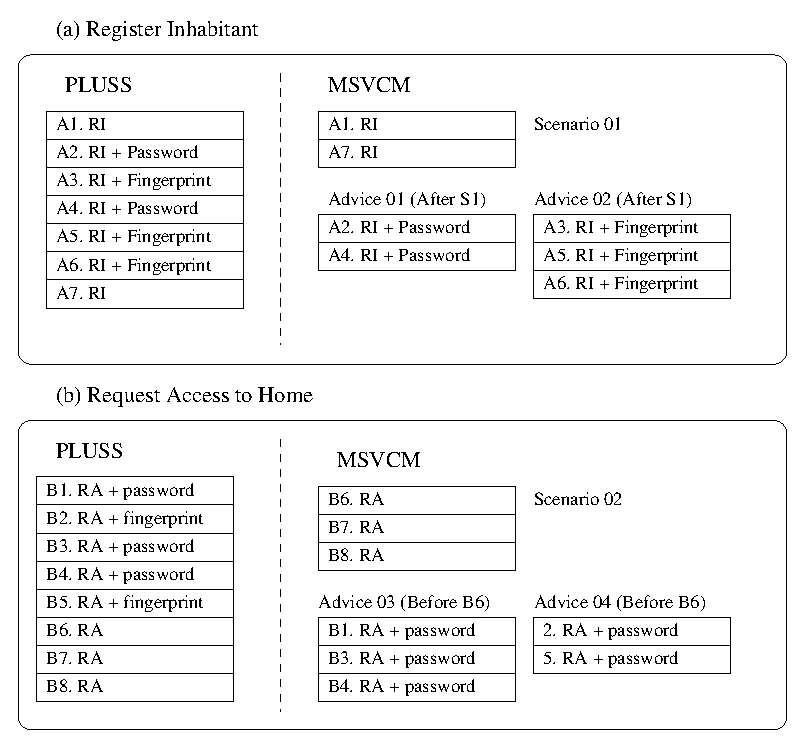
\includegraphics[scale=0.60]{img/comparisonScenarios.eps}
  \caption{Sample of Smart Home assignment.}
  \label{fig:smartHomeScenarios}
  \end{center}
\end{figure}

Similarly, Figure~\ref{fig:MMSScenarios} shows some feature assignments for the
MMS product line. In this case, we want to emphasize that the behavior related to
the \emph{Store an Embedded Number} and \emph{Send a Message to Embedded Email} 
features change the behavior of the \emph{Receive a MMS} (RM) and \emph{Select a
MMS for Displaying} (SM) features in a similar way. For this reason, we
classify the behavior of the \emph{Store an Embedded Number} and \emph{Send
a Message to Embedded Email} features as \emph{homogeneous}. On the other hand,
we say that the \emph{Password} optional feature of the Smart Home case study has a
\emph{heterogeneous crosscutting behavior}, since its specification could not be
modularized in a unique advice (Figure~\ref{fig:smartHomeScenarios}(a) and
(b)). The same occurred with the \emph{Fingerprint} feature.

\begin{figure}[bth]
 \begin{center}
  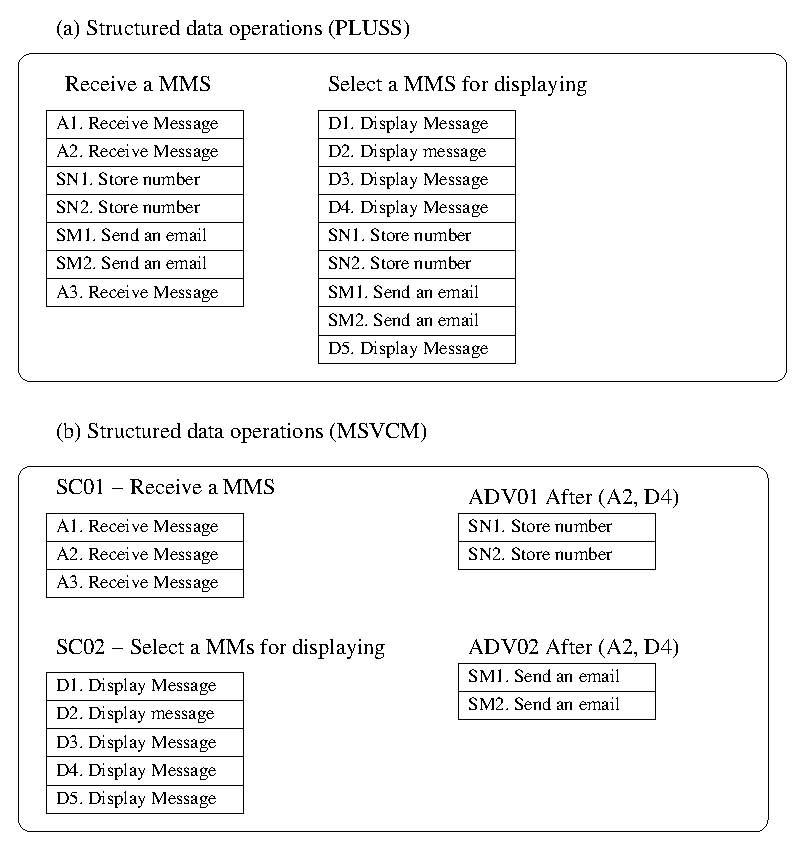
\includegraphics[scale=0.60]{img/comparisonScenarios2.eps}
  \caption{Sample of MMS assignment.}
  \label{fig:MMSScenarios}
  \end{center}
\end{figure}

We have observed that the \emph{crosscutting nature} of a feature, which here we
consider as being homogeneous or heterogeneous, has a great influence in our
results. For instance, Table~\ref{tab:feature-dos} shows the DoS of
the assets depicted in Figures~\ref{fig:smartHomeScenarios}
and~\ref{fig:MMSScenarios}. Notice that, in MSVCM, modularizing the behavior
of \emph{Password} and \emph{Fingerprint} as advices had
increased the DoS of both \emph{Register Inhabitant} and \emph{Request Access to
Home} features. This side effect does not occur with homogeneous
crosscutting features--- modularizing the
\emph{Store a Number} and \emph{Send Message to Email} as advices does not 
change the DoS of the \emph{Receive a MMS} and \emph{Display a MMS} features.    

\begin{table}[htb]
\centering
\caption{DoS of the presented features}
\label{tab:feature-dos}
\begin{small}
\begin{tabular}{llll} \hline
SPL							&	Feature							& PLUSS	& MSVCM	\\ \hline 
\multirow{4}{*}{Smart Home} &	Register Inhabitant				& 0.00  & 0.57  \\
							&	Request Access to Home			& 0.00  & 0.57  \\ 
							&	Password						& 0.96  & 0.78  \\ 
							&	Fingerprint						& 0.96  & 0.78  \\ \hline
\multirow{4}{*}{MMS} 		&	Receive a MMS					& 0.00  & 0.00  \\ 
							&	Display a MSS					& 0.00  & 0.00  \\ 
							& 	Store a Number					& 1.00  & 0.00  \\
							& 	Send Message to Email			& 1.00  & 0.00  \\ \hline		
\end{tabular}
\end{small}
\end{table}

Besides that, independently of the crosscutting nature of a feature, the
MSVCM approach eliminates the tangling of the base scenarios, quantified by
the DoF metric. As shown in Table~\ref{tab:scenario-dof}, the base scenarios in
MSVCM have a higher degree of focus. 

In what follows, we present summaries of the data collected from the
aforementioned case studies. Since each case study presents a different distribution of
\emph{crosscutting features}, the significance level related to the benefits
of our approach vary. All specifications and collected data are available at
the \emph{Software and Process} area of a web site~\cite{SPG:site}.


\begin{table}[htb]
\centering
\caption{DoF of the presented scenarios}
\label{tab:scenario-dof}
\begin{small}
\begin{tabular}{llll} \hline
SPL							&	Scenario		& PLUSS	& MSVCM	\\ \hline
\multirow{2}{*}{Smart Home} &	Scenario 01		& 0.24  & 1.00  \\
							&	Scenario 02		& 0.27  & 1.00  \\ \hline
\multirow{2}{*}{MMS} 		&	Scenario 01		& 0.12  & 1.00  \\ 
							&	Scenario 02		& 0.20  & 1.00  \\ \hline
\end{tabular}
\end{small}
\end{table}

}

\subsection{Smart Home assessment}

This study aimed at comparing feature modularity of PLUSS and MSVCM
specifications. Initially, three different products of the security module of a
Smart Home family~\cite{Pohl:2005aa} were specified. Almost six use cases and
fifteen scenarios are present in each product, with a significant number of
duplicated steps among them. These specifications, available on-line, were used
as input data. Then, six students, organized in groups, were assigned to identify
the commonalities and variabilities among the products, and to restructure the
input specifications. Two SPL specifications were produced, one using the PLUSS
notation and the other one using the MSVCM approach

%This study was divided in four major phases: (1) the specification of the input
%data --- three different configurations of the security module of a smart home
%were specified without PL support; (2) the presentation of preparatory classes to the subjects
%(graduate students with similar skills in the area); (3) the activity of
%restructuring the input specifications using both PLUSS and the Crosscutting
%technique; and (4) the assessment of the resulting specifications.
%In the first phase we have specified three different configurations of the
%security module of a Smart Home. These specifications included feature models and
%use case scenarios written without product line support. Additionally, they were
%build upon the documentation available from~\cite{Pohl:2005aa,AMPLE}.

%In the second phase, introductory classes and bibliographic references were
%offered to post-graduate students. At that period, none of these students had had
%previous knowledge in the field of scenario variability management. A total of
%six students were involved in this case study. Then, the students were organized
%in groups and assigned to restructure the input specifications using PLUSS and
%Crosscutting techniques.


Table~\ref{tab:sh-dos} summarizes the resulting \emph{degree of scattering} of
the Smart Home features, computed from the PLUSS and MSVCM specifications.
Although the MSVCM approach achieved a central tendency (median) of DoS closer to
zero, we can not realize any significant improvement in this metric. Actually,
for some features (3 features in a total of 17), the DoS for the MSVCM approach
presented a greater value than the corresponding ones in PLUSS.


\begin{table}[htb]
\centering
\caption{Smart Home degree of scattering}
\label{tab:sh-dos}
\begin{small}
\begin{tabular}{llllll} \hline
					& Min 	& Median 	& Mean 	& Max 	& St. Deviation \\ \hline \\
	PLUSS			& 0.00  & 0.26   	& 0.28  & 0.70 	& 0.08 			\\
	MSVCM	& 0.00  & 0.00  	& 0.26 	& 0.82 & 0.10  		\\ \hline	
\end{tabular}
\end{small}
\end{table}

As discussed in the previous section, modularizing the variant behavior of
\emph{Register Inhabitant} and \emph{Request Access to Home} in aspectual
scenarios produced the side effect of increasing the DoS, at the same time that it reduced
the tangling of the related scenarios. On the other hand, the feature \emph{Turn
On Internal and External Lights} presents a lower DoS in the MSVCM approach
(0.00) when compared to the PLUSS (0.54) notation. This feature requires a
behavior that crosscuts, in a homogeneous way, the different scenarios related to
the $Intrusion\ Detection$ use case.


Considering the degree of focus (data summarized in Table~\ref{tab:sh-dof}), we
have evidences of a significant improvement of the MSVCM approach
(\emph{p-value=0.06}). Notice that the central tendency (median) of DoF in the
MSVCM approach ($1.00$) is closer to one than the corresponding value
($0.63$) in the PLUSS notation.

\begin{table}[htb] \centering
\caption{Smart Home degree of focus}
\label{tab:sh-dof}
\begin{small}
\begin{tabular}{llllll} \hline
					& Min 	& Median 	& Mean 	& Max 	& St. Deviation \\ \hline \\
	PLUSS			& 0.33  & 0.63   	& 0.68  & 1.00 	& 0.07 			\\
	MSVCM			& 0.35  & 1.00   	& 0.82 	& 1.00 	& 0.05			\\ \hline	
\end{tabular}
\end{small}
\end{table}

Describing all variants of a behavior in a single asset
(as exemplified in Section~\ref{sec:problem}) is the main reason for the lack of
focus in scenarios written in the PLUSS approach. On the other hand, the MSVCM technique
allows the modularization of variant behavior in aspectual scenarios. The result
is a better separation between common and optional steps of a scenario.

% {\color{green}In summary, the Smart Home case study gives us some evidences that
% removing tangling by means of aspectual scenarios improves the \emph{degree of focus}.
% Moreover, if the variant steps of a scenario corresponds to a homogeneous
% crosscutting behavior, modularizing it as an aspectual scenario also improves the
% DoS. On the other hand, modularizing features effected by heterogeneous
% crosscutting behavior increases the corresponding \emph{degree of scattering}, at
% the same time that it reduces the tangling of base scenarios.}


%The next sections present the evaluation of the Pedagogical Product Line (PPL)
%and Multimedia Message Product Line (MMS). We have compared our specification of
%\emph{MMS} product line to the specifications we had written for the
%PLUSS technique. Similarly, we have compared our specification
%of the PPL to a specification that had been sent to us by
%the authors of the PLUSS approach.

\subsection{MMS assessment}

As explained earlier, the MMS product line, which was adapted from an industrial
partner, enables the customization of multimedia message applications. The
primary goal of each one of these applications is to create and send messages
with embedded multimedia content (image, audio, video)~\cite{Bonifacio:2008aa}.
We have specified the MMS product line using both Crosscutting and PLUSS
techniques. The results of this case study are
summarized in Tables~\ref{tab:mms-dos}~and~\ref{tab:mms-dof}.

\begin{table}[htb] \centering
\caption{MMS degree of scattering}
\label{tab:mms-dos}
\begin{small}
\begin{tabular}{llllll} \hline
					& Min 	& Median 	& Mean 	& Max 	& St. Deviation \\ \hline \\
	PLUSS			& 0.00  & 0.60   	& 0.46  & 0.80 	& 0.11 			\\
	MSVCM			& 0.00  & 0.41   	& 0.34 	& 0.79 	& 0.10			\\ \hline	
\end{tabular}
\end{small}
\end{table}

This case study, differently from the Smart Home, gives evidence of improvements of the
MSVCM approach with respect to the feature's \emph{degree of scattering}
(\emph{p-value=0.01}). This result was mainly achieved because several of the features of
the MMS product line require a homogeneous crosscutting behavior. For example,
there are some policies related to DRM\footnote{Digital Rights Management}
content that crosscut, in a uniform manner, the behavior related to
\emph{sending} and \emph{forwarding} messages.

On the other hand, the MMS case study didn't reveal significant improvements with
respect to the \emph{degree of focus} metric (Table~\ref{tab:mms-dof}). This
result is also different from the corresponding one observed in the Smart Home
case study. The main reason for such a difference is that several scenarios of
the Smart Home specification are effected by alternative features. On the other
hand, just a few scenarios of the MMS case study are effected by alternative
features. Thus, the benefits achieved from extracting varying behavior to
aspectual scenarios were minimized in this case study.

\begin{table}[htb] \centering
\caption{MMS degree of focus}
\label{tab:mms-dof}
\begin{small}
\begin{tabular}{llllll} \hline
					& Min 	& Median 	& Mean 	& Max 	& St. Deviation \\ \hline \\
	PLUSS			& 0.34	& 0.59		& 0.70	& 1.00	& 0.07			\\
	MSVCM			& 0.46  & 0.59   	& 0.71 	& 1.00 	& 0.06			\\ \hline	
\end{tabular}
\end{small}
\end{table}

\subsection{PPL assessment}

We compared our approach to a PPL specification that was sent to us by the
authors of the PLUSS technique. Similarly to the Smart Home product line, the PPL has been used in several case
studies in the area. The original specification of PPL~\cite{PPL:2008} is already well
modularized, since its features, in general, do not crosscut different
use cases. Moreover, another characteristic of the PPL is that several features
are related to qualities that do not effect scenario specifications.
Even in this context, our approach achieves some improvements in the
resulting \emph{degree of scattering} (Table~\ref{tab:ppl-dos}). For instance,
in almost all features we were able to improve the DoS (\emph{p-value=0.008}).


\begin{table}[htb] \centering
\caption{PPL degree of scattering}
\label{tab:ppl-dos}
\begin{small}
\begin{tabular}{llllll} \hline
					& Min 	& Median 	& Mean 	& Max 	& St. Deviation \\ \hline \\
	PLUSS			& 0.00	& 0.48		& 0.32	& 0.71	& 0.08			\\
	MSVCM			& 0.00  & 0.00   	& 0.07 	& 0.64 	& 0.05			\\ \hline	
\end{tabular}
\end{small}
\end{table}


Modularizing the error handling feature was the main reason for the
aforementioned improvement. By applying our approach, all behavior related to
the \emph{error handling} concern was modularized in a single scenario. The
composition of \emph{error handling} with the basic scenarios was done by means
of annotations to the corresponding steps. For instance,
Figure~\ref{fig:error-handle} depicts just one scenario for error handling:
raising  an error when there is no space available in the file system.


\begin{figure}[h]
\begin{scriptsize}
\texttt{
\begin{tabular}{l}
     Description: There is no available space in file system.\\
     After: [CatchFileException] \\
\end{tabular}
\begin{center}
\begin{tabular}{|p{0.1in}|p{0.6in}|p{1.0in}|p{1.0in}|} \hline
Id & User Action & System State & System Response \\ \hline \hline
E1 & & There is not enough space to save the file. &  Raise the Disk is Full exception. The arcade game application is finished. \\  \hline \end{tabular} \end{center} }
\end{scriptsize}
\caption{Error handling scenario.}
\label{fig:error-handle}
\end{figure}

This scenario can be started from any step that has been marked with
the \emph{CatchFileException} annotation.
Several features of the PPL need to save information in the file system.
Therefore, in the PLUSS specifications of the \emph{Pedagogical}
Product Line, several use cases have to deal with this kind of exception.
As a consequence, we achieve a reduction (almost 20\%) in the number of scenario
steps when compared to the PLUSS approach.

%It is important to notice that this
%reduction of size didn't compromise the requirements coverage; it actually
%represents an improvement in specification reuse.

On the other hand, we
didn't get improvements in the \emph{degree of focus} metric
(Table~\ref{tab:ppl-dof}). Again, this result is primarily motivated by the
reason that just a few scenarios of PPL are effected by alternative features. 

\begin{table}[htb] \centering
\caption{PPL degree of focus}
\label{tab:ppl-dof}
\begin{small}
\begin{tabular}{llllll} \hline
					& Min 	& Median 	& Mean 	& Max 	& St. Deviation \\ \hline \\
	PLUSS			& 0.44	& 1.00		& 0.78	& 1.00	& 0.07			\\
	MSVCM	& 0.44  & 1.00   	& 0.83 	& 1.00 	& 0.07			\\ \hline	
\end{tabular}
\end{small}
\end{table}

\subsection{Discussion}

{\color{red} After running the different case studies, we concluded that the 
\emph{greater} is the number of \emph{homogeneous crosscutting features} and
the number of alternatives for a same behavior, the greater is the 
benefits of applying our approach. In that cases, the MSVCM improvements of 
both feature modularity and scenario cohesion become more evident. 

In fact, the expected benefit of our approach is to reduce the impact of
evolving a SPL. If a scenario has a lower DoF, introducing a new alternative to its variant behavior
requires more changes in the base specification. On the other hand, the level of
modularity supported by our approach reduces the number of changes in the base
scenarios of a SPL. As a consequence, a SPL evolves by means of the
introduction of new scenarios and/or advices. Additionally, evolving a feature
with lower DoS require changes in localized assets.  

Investigating the effort required for specifying a SPL in
PLUSS and MSVCM is an issue for future research. However, it is important
to note that SPL development, independently of the approach, requires a
mapping between the domain and solution spaces~\cite{Czarnecki:2000aa}. As a
consequence, here we do not introduce new kinds of concerns to the SPL
development. Actually, our approach just presents a better separation for
mapping those SPL concerns. }


% \subsection{DSM Analysis}
% 
% In this section we apply \emph{Design Structure Matrices} (DSMs) to report on the
% benefits of a clear separation between variability management and scenarios
% specifications. A DSM is a tool for visualizing dependencies between design
% decisions~\cite{Baldwin:2000aa}. Such decisions are arranged in both columns and
% rows of a matrix. Using the terminology described in~\cite{Czarnecki:2000aa}, the
% design decisions that we consider in this analysis are related to the problem
% space (represented as feature models), the solution space (represented as the use
% case models), the configuration space (used to relate the problem space to the
% solution space), and the product configurations.
% 
% 
%  We can identify dependencies between design decisions by observing the columns
%  in a given row~\cite{Baldwin:2000aa}. For example, the first row in
%  Figure~\ref{dsm:pluc} indicates that the task of creating the problem space in
%  PLUC depends on the task of creating the solution space. The first can not be
%  independently performed before the second. As presented in
%  Section~\ref{sec:problem}, the PLUC approach describes product instances and
%  variability space at specific sections of use cases. Therefore, it is not
%  possible to evolve variability management (introducing new variants of existing
%  features, products, or relations between features and artifacts) without
%  reviewing the use case model. This is expressed in the non modular DSM of
%  Figure~\ref{dsm:pluc}, which depicts cyclical dependencies between the problem
%  space and the solution space.
% 
% 
% \begin{figure}[htb]
% \centering
% \begin{small}
% \begin{tabular}{llllll} \hline
%   &                         & 1 & 2 & 3 & 4 \\ \hline
% 1 & Problem space           &   & x &   &   \\
% 2 & Solution space          & x &   & x & x \\
% 3 & Configuration space     & x & x &   &   \\
% 4 & Product configuration   & x & x &   &   \\ \hline
% \end{tabular}
% \end{small}
% \caption{DSM Analysis of PLUC}
% \label{dsm:pluc}
% \end{figure}
% 
% PLUSS partially solves (see Figure~\ref{dsm:pluss}) the cyclical dependencies just presented, since the problem space is not documented in the same artifact of the solution space. However, since there is no independent model used to relate features to use cases, PLUSS still presents a cyclical dependency between the solution space and the configuration space. As a consequence, it is not possible to independently evolve the configuration space without reviewing existing scenarios.
% 
% \begin{figure}[htb]
% \centering
% \begin{small}
% \begin{tabular}{llllll} \hline
%   &                         & 1 & 2 & 3 & 4 \\ \hline
% 1 & Problem space           &   &   &   &   \\
% 2 & Solution space          & x &   & x &   \\
% 3 & Configuration space     & x & x &   &   \\
% 4 & Product configuration   & x &  &   &    \\ \hline
% \end{tabular}
% \end{small}
% \caption{DSM Analysis of PLUSS}
% \label{dsm:pluss}
% \end{figure}
% 
% Our approach reduces the dependencies between variability management and scenario specifications
% (Figure~\ref{dsm:cc}). For instance, introducing new alternatives of a feature does not require changes in the existing scenarios. Notice that the proposed configuration knowledge, used to relate feature expressions to artifacts, is responsible for
% decoupling the solution space from the configuration space.
% 
% \begin{figure}[h]
% \centering
% \begin{small}
% \begin{tabular}{llllll} \hline
%   &                         & 1 & 2 & 3 & 4 \\ \hline
% 1 & Problem space           &   &   &   &   \\
% 2 & Solution space          & x &   &   &   \\
% 3 & Configuration space     & x & x &   &   \\
% 4 & Product configuration   & x &  &    &    \\ \hline
% \end{tabular}
% \end{small}
% \caption{DSM Analysis of MSVCM}
% \label{dsm:cc}
% \end{figure}


%===========================
% Related work
%===========================
\section{Related Work}
\label{sec:related}

Several approaches have been proposed for representing
scenario variability~\cite{Jacobson:1997aa,Griss:1998aa, Eriksson:2005aa,Bertolino:2003aa}. However, in this paper
we only compare our crosscutting approach with PLUC and
PLUSS techniques because they encompass a broad range
of SoC between variability management and scenario specifications.
PLUC presents the lowest level of modularity, since
almost all information related to variability is tangled within
use cases. Although PLUSS partially reduces such a tangling,
by considering the importance of feature modeling, some
dependencies from scenarios to features are still present.

Regarding to the early representation of aspects, there are works proposed to
represent weaving mechanisms for textual
requirements~\cite{Chitchyan:2007aa,Sillito:2004aa}. Our work also supports the
composition of aspects and scenarios specifications. However, differently from
the previous works, our mechanisms were proposed for variability management, and
considers the effect of different languages used in the SPL domain (such as
feature models, configuration knowledge, and product configurations). Other works
were proposed in order to represent weaving mechanisms using abstract state
machines and activity
diagrams~\cite{Noda:2006aa,Cottenier:2006aa,Alferez:2008aa}. Our decision for
using textual specifications was motivated because this notation is widely used
in industry~\cite{Denger:2001aa} and our industrial partner uses
textual scenarios as input for generating test artifacts.


Another difference of our work, comparing it with existing proposals for the
early specification of crosscutting concerns, is that the semantics of our
weavers are expressed using a well defined notion of crosscutting mechanisms.


In order to avoid the problem of \emph{fragile pointcuts}, Chitchyan
et al. proposed a semantic approach for scenario
composition~\cite{Chitchyan:2007aa}. Such an approach is based on
natural language processing. Using our \emph{evaluateAspect} weaver
(Section~\ref{sub:sc-weaver}), \emph{pointcuts} can be
defined using either references to \emph{step ids} or references to \emph{step annotations};
which, although being more invasive, also reduces the problem of \emph{fragile pointcut}. However, this is an orthogonal problem. We are able to introduce semantic based compositions by implementing the corresponding algorithm in the \emph{match} function, which is used in the reference implementation of  discussed in Section~\ref{sub:sc-weaver}).

Metrics for quantifying scattering and tangling~\cite{Eaddy:2007aa,Figueiredo:2008aa} and
Design Structure Matrices (DSMs)~\cite{Sullivan:2005aa,Lopes:2006aa}
have been applied for assessing modularity in aspect-oriented
systems. In this work, we applied
DSMs in the context of scenario variability management.
Moreover, we customized a suite of metrics for quantifying
the degree of scattering of features and the degree of focus of scenarios.
To our knowledge, our work is unique in applying both DSMs and crosscutting metrics for evaluating SoC in scenario variability.


%========================
% Conclusions
%========================
\section{Conclusions}\label{sec:conclusions}

In this paper we formally described variability management as a
crosscutting mechanisms, considering the contribution
of different input languages that crosscut each other for deriving
specific members of a product line.

We applied this notion of variability management in the context of use
case scenarios, achieving several benefits. 
First, our approach supports
a clear separation of concerns between variability and scenario specifications,
allowing both representations to evolve independently. Second, for different case studies we improve both feature modularity and scenario cohesion. Finally, we achieved a reduction in the size of specifications by composing scenarios in a quantified way. 

Although our modeling framework was instantiated for representing
scenario variabilities, we believe that it could be applied to
other SPL artifacts. Particularly, optional and parameterized artifacts
are also relevant for non-functional requirements and test cases.
Moreover, our notion of crosscutting was based on a work target at source code definitions of crosscutting. Therefore,
we argue that representing variabilities in source code, using our modeling framework,
is straightforward.

%As future work, we would like to apply our notion of variability management in order
%to identify relationships between
%variabilities at different SPL artifacts (in a first moment, relationships between
%requirements and test artifacts). Such kind of relationships can help in the product
%generation and traceability activities of a SPL.
%The modeling
%framework proposed in this work takes a step in this direction, since the
%composition process used to derive product specific scenarios have been formally represented. 

%
% ---- Bibliography ----
%

\bibliographystyle{abbrv}
\bibliography{../references/phd-references}


\end{document}
